\label{sec:hadhad_multijet}

Multi-jet production is a source of background in the \hadhad signal
region where both \tauhadvis candidates originate from the
misidentification of quark- or gluon-initiated jets. It represents the
second largest background with \faketauhadvis in the \hadhad SR after
the dominant \ttbarFakes contribution.

\subsubsection{The fake factor method}

The multi-jet background is estimated using the fake factor method
which is a data-driven method for background estimation. It is
applicable in cases where two event observables exist that are
statistically independent for the background process to be estimated,
while also being strong discriminators between the background and
other processes (signal and non-multi-jet processes). Four disjoint
regions can be defined, three background-enriched control regions and
a signal-like region, by performing a binary categorisation of each
observable. The assumption of statistical independence allows to
relate the expected number of events for the background process
between the control regions and the signal-like region, thus yielding
a data-driven estimate of the expected background contribution in the
signal-like region.

In the \hadhad channel, two observables that allow to define control
regions enriched in multi-jet events are the \tauid requirements
fulfilled by the \tauhadvis candidates and the sign of the electric
charges of both candidates.

In the signal region, \tauhadvis candidates are required to pass the
loose \tauid working point. This requirement defines regions where
both \tauhadvis candidates pass identification, herafter referred to
as ID regions. The selection is partially inverted to obtain control
regions enhanced in multi-jet events by requiring that exactly one
\tauhadvis candidate is failing the loose \tauid working point while
still passing a working point corresponding to an efficiency loss of
\tauhad of about 1\,\% ($\text{RNN score} > 0.01$). The \tauhadvis
candidates fulfilling this selection are referred to as
anti-\tauhadvis and the regions defined by the inversion of the
identification criterion as Anti-ID regions. The identification
criterion cannot be fully inverted due to pre-selections\footnote{In
  the ATLAS collaboration, datasets targeting $\PHiggs \to \hadhad$
  processes require events with at least one \tauhadvis passing the
  loose \tauid working point and one \tauhadvis with a \tauid score
  exceeding 0.01.} applied in the data reduction pipeline of the ATLAS
experiment. However, the fake factor method is still valid in the
presence of these constraints provided the underlying assumptions of
the method hold.

The electric charge of both \tauhadvis candidates produced from signal
processes and dominant sources of backgrounds with two \tauhadvis
orginating for hadronic $\tau$~decays ($\PZ \to \tautau$,
$\PHiggs \to \tautau$, \ttbar) are expected to be reconstructed with
opposite-sign (OS) electric charge. The OS requirement is inverted
yielding regions with \tauhadvis candidates of same-sign (SS) electric
charge, depleting the region of processes where both \tauhadvis
orginate from hadronic $\tau$ decays. In contrast, the multi-jet
background contributes similarly to the OS and SS regions since
\tauhadvis charge reconstruction has little sensitivity to the
relative sign of the electric charge between partons initiating jets
that are being misidentified as \tauhadvis.

With the previously defined control regions and the assumption of
independence of the observables defining the regions, the expected
multi-jet contribution in regions with \tauhadvis passing loose
identification and with \tauhadvis pairs of opposite-sign electric
charge can be estimated using
\begin{align*}
  N_\text{multi-jet}^{\text{OS, ID}} =
  N_\text{multi-jet}^{\text{OS, Anti-ID}}
  \cdot
  \underbrace{\frac{N_\text{multi-jet}^{\text{SS, ID}}}
  {N_\text{multi-jet}^{\text{SS, Anti-ID}}}}
  _{= \text{FF}_\text{SS}} \,\text{,}
\end{align*}
where $N_\text{multi-jet}$ is the number of multi-jet events in a
given region. The fake factor (FF) measures the ratio of multi-jet
events in the ID and Anti-ID region\footnote{The use of identification
  or isolation criteria to define the ratio is the main difference
  between the fake factor method and the more general ABCD method.}.

The control regions defined by inverting the OS and/or ID requirements on
\tauhadvis do not provide pure samples of multi-jet events. Therefore,
number of multi-jet events is estimated according to
\begin{align*}
  N_\text{multi-jet} = N_\text{data} - N_\text{non-multi-jet} \,\text{,}
\end{align*}
where $N_\text{data}$ is the observed number of events in the
multi-jet enriched region and $N_\text{non-multi-jet}$ the expected
contribution of non-multi-jet events estimated using simulation.

The probability of misidentifying a quark- or gluon-jet as a hadronic
$\tau$ decay depends on the properties of the reconstructed \tauhadvis
candidate. Particularly, the reconstructed decay mode and visible
transverse momentum affect the probability of a jet reconstructed as a
\tauhadvis to pass \tauid (cf.\ \Cref{sec:tauid}). To control for this
effect, the fake factor method is performed in bins of observables related
to the properties of reconstructed \tauhadvis.

In~\Cref{tab:mjfakes_yields} the multi-jet and non-multi-jet yields in
the regions relevant for the \faketauhadvis estimation are
summarised. The 2 $b$-tag region, while most similar to the signal
region, is not well suited to estimate fake factors:
\begin{itemize}

\item The 2 $b$-tag regions used for the measurement of fake factors
  have a large contamination from non-multi-jet backgrounds, primarily
  \ttbarFakes, that have to be subtracted. The large size of the
  subtraction leads to a degradation of the statistical precision of
  measured fake factors and inflates systematic uncertainties
  originating from the modelling of the subtracted components.

\item The strict \btag requirement suppresses the multi-jet
  contribution in the control regions preventing a differential
  measurement of fake factors in properties of the \tauhadvis.

\item The multi-jet estimate cannot be validated in the 2 $b$-tag
  region due to the absence of a region with high multi-jet purity
  that is similar to the signal region.

  % Resultingly, the statistical independence of the charge sign and ID
  % observables employed by the FF method cannot be verified.
\end{itemize}
These issues are addressed by performing the fake factor measurement
in the 1 $b$-tag region instead, which has a higher abundance and
purity of multi-jet events, and extrapolating the measurement into the
2 $b$-tag region to obtain a multi-jet background estimate in the
signal region. Distributions of the \pT of the leading and sub-leading
\tauhadvis candidates in the regions relevant to the fake factor
measurement are shown in~\Cref{fig:mjfakes_1tag_ss_plots}.

\begin{table}[htbp]
  \centering

  \begin{subtable}[t]{\textwidth}
    \centering
    % Size of subtraction and multi-jet purity:
%                         multi_jet  non_multi_jet  multi_jet_error  non_multi_jet_error  multi_jet_purity
% anti_id charge_sign
% False   OS           16067.048497   16443.951503       204.558258            96.607872          0.494203
%         SS           14040.394005    1971.605995       129.147367            25.827164          0.876867
% True    OS           91582.182374   13677.817626       334.090987            79.729466          0.870057
%         SS           78399.983641    5707.016359       296.470480            61.544664          0.932146

\begin{tabular}{
  ll
  S[table-format=5.0(3)]
  S[table-format=5.0(3)]
  c}
  \toprule
  \multicolumn{2}{l}{Region} & {$N_\text{multi-jet}$} & {$N_\text{non-multi-jet}$} & {Multi-jet purity} \\
  \midrule
  \multirow{2}{*}{SS} & ID      & 14040 +- 130 & 1970 +- 30   & 88\,\% \\
                      & Anti-ID & 78400 +- 300 & 5710 +- 70   & 93\,\% \\
  \midrule
  \multirow{2}{*}{OS} & ID      & 16070 +- 210 & 16440 +- 100 & 49\,\% \\
                      & Anti-ID & 91580 +- 340 & 13680 +- 80  & 87\,\% \\
  \bottomrule
\end{tabular}



%%% Local Variables:
%%% mode: latex
%%% TeX-master: "../phd_thesis"
%%% End:

    \subcaption{1 $b$-tag regions}
    \label{tab:mjfakes_yields_1tag}
  \end{subtable}

  \begin{subtable}[t]{\textwidth}
    \centering
    % Size of subtraction and multi-jet purity:
%                        multi_jet  non_multi_jet  multi_jet_error  non_multi_jet_error  multi_jet_purity
% anti_id charge_sign
% False   OS            408.197943    7971.802057       105.950917            53.344135          0.048711
%         SS           1299.622259    1001.377741        50.345854            15.287412          0.564808
% True    OS           8429.603396    8864.396604       139.699303            47.136984          0.487429
%         SS           7653.735896    3338.264104       108.557939            28.157166          0.696301

\begin{tabular}{
  ll
  S[table-format=5.0(3)]
  S[table-format=5.0(3)]
  c}
  \toprule
  \multicolumn{2}{l}{Region} & {$N_\text{multi-jet}$} & {$N_\text{non-multi-jet}$} & {Multi-jet purity} \\
  \midrule
  \multirow{2}{*}{SS} & ID      & 1300 +- 60  & 1000 +- 20 & 56\,\% \\
                             & Anti-ID & 7650 +- 110 & 3340 +- 30 & 70\,\% \\
  \midrule
  \multirow{2}{*}{OS} & ID      & \multicolumn{3}{c}{\rule[3pt]{5.2em}{0.3pt}\hspace{1em}Signal Region\hspace{1em}\rule[3pt]{5.2em}{0.3pt}} \\
                             & Anti-ID & 8430 +- 140 & 8860 +- 50 & 49\,\% \\
  \bottomrule
\end{tabular}




%%% Local Variables:
%%% mode: latex
%%% TeX-master: "../phd_thesis"
%%% End:

    \subcaption{2 $b$-tag regions}
  \end{subtable}

  \caption{Number of multi-jet events in regions defined by the
    electric charge of the \tauhadvis pair (OS, SS) and \tauhadvis
    identification (ID, Anti-ID). The number of multi-jet events,
    $N_\text{multi-jet}$, is estimated by subtracting the number
    non-multi-jet events, $N_\text{non-multi-jet}$, estimated using
    Monte Carlo simulation from the observed number of events in this
    region. The breakdown is shown after the 1 $b$-tag requirement in
    (a); after the 2 $b$-tag requirement in (b). The signal region (2
    $b$-tag OS ID) is omitted. Uncertainties are from data and MC
    statistical sources only.}
  \label{tab:mjfakes_yields}
\end{table}

\begin{figure}[htbp]
  \centering

  \begin{subfigure}{0.49\textwidth}
    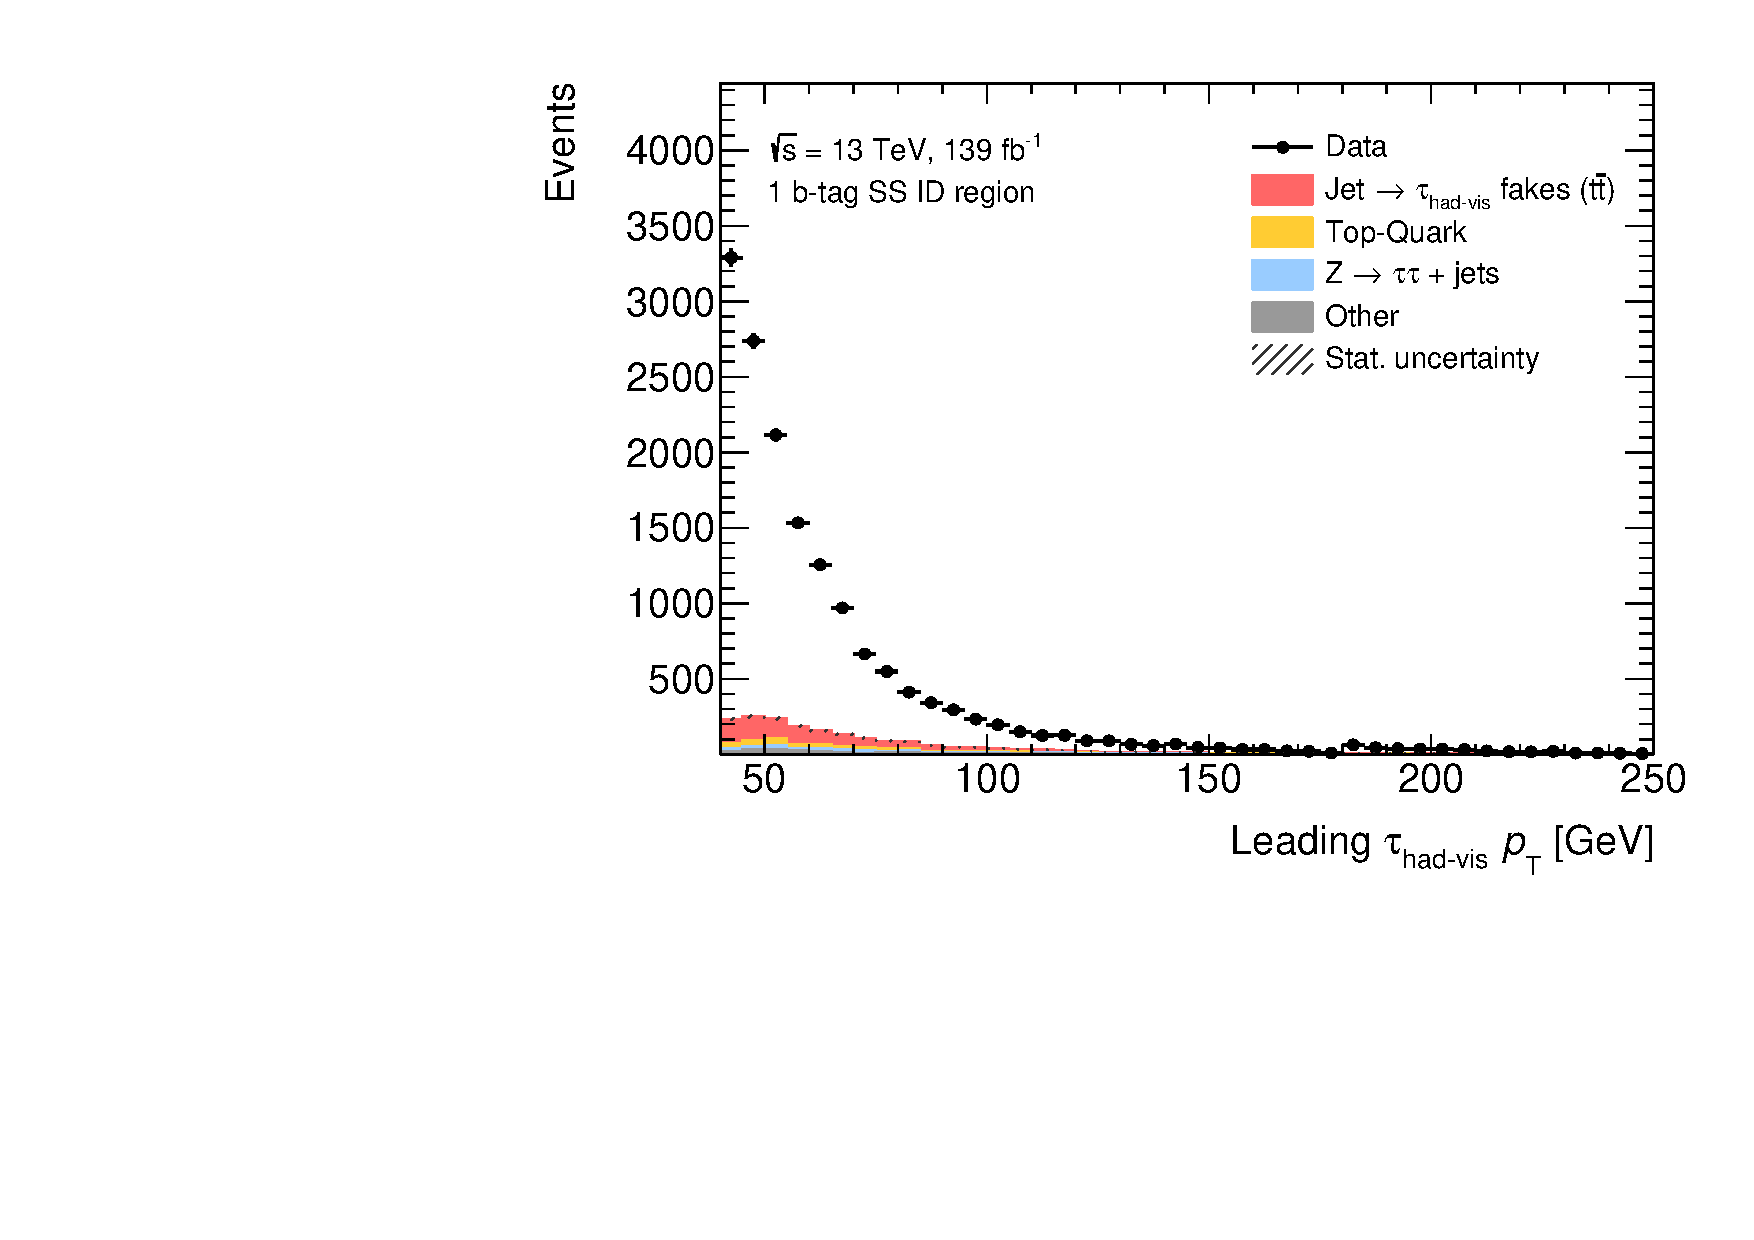
\includegraphics[width=\textwidth]{fakefactors/region_plots/tau0pt_1tag_ss_id}
    \subcaption{1 $b$-tag SS ID region}
  \end{subfigure}
  \begin{subfigure}{0.49\textwidth}
    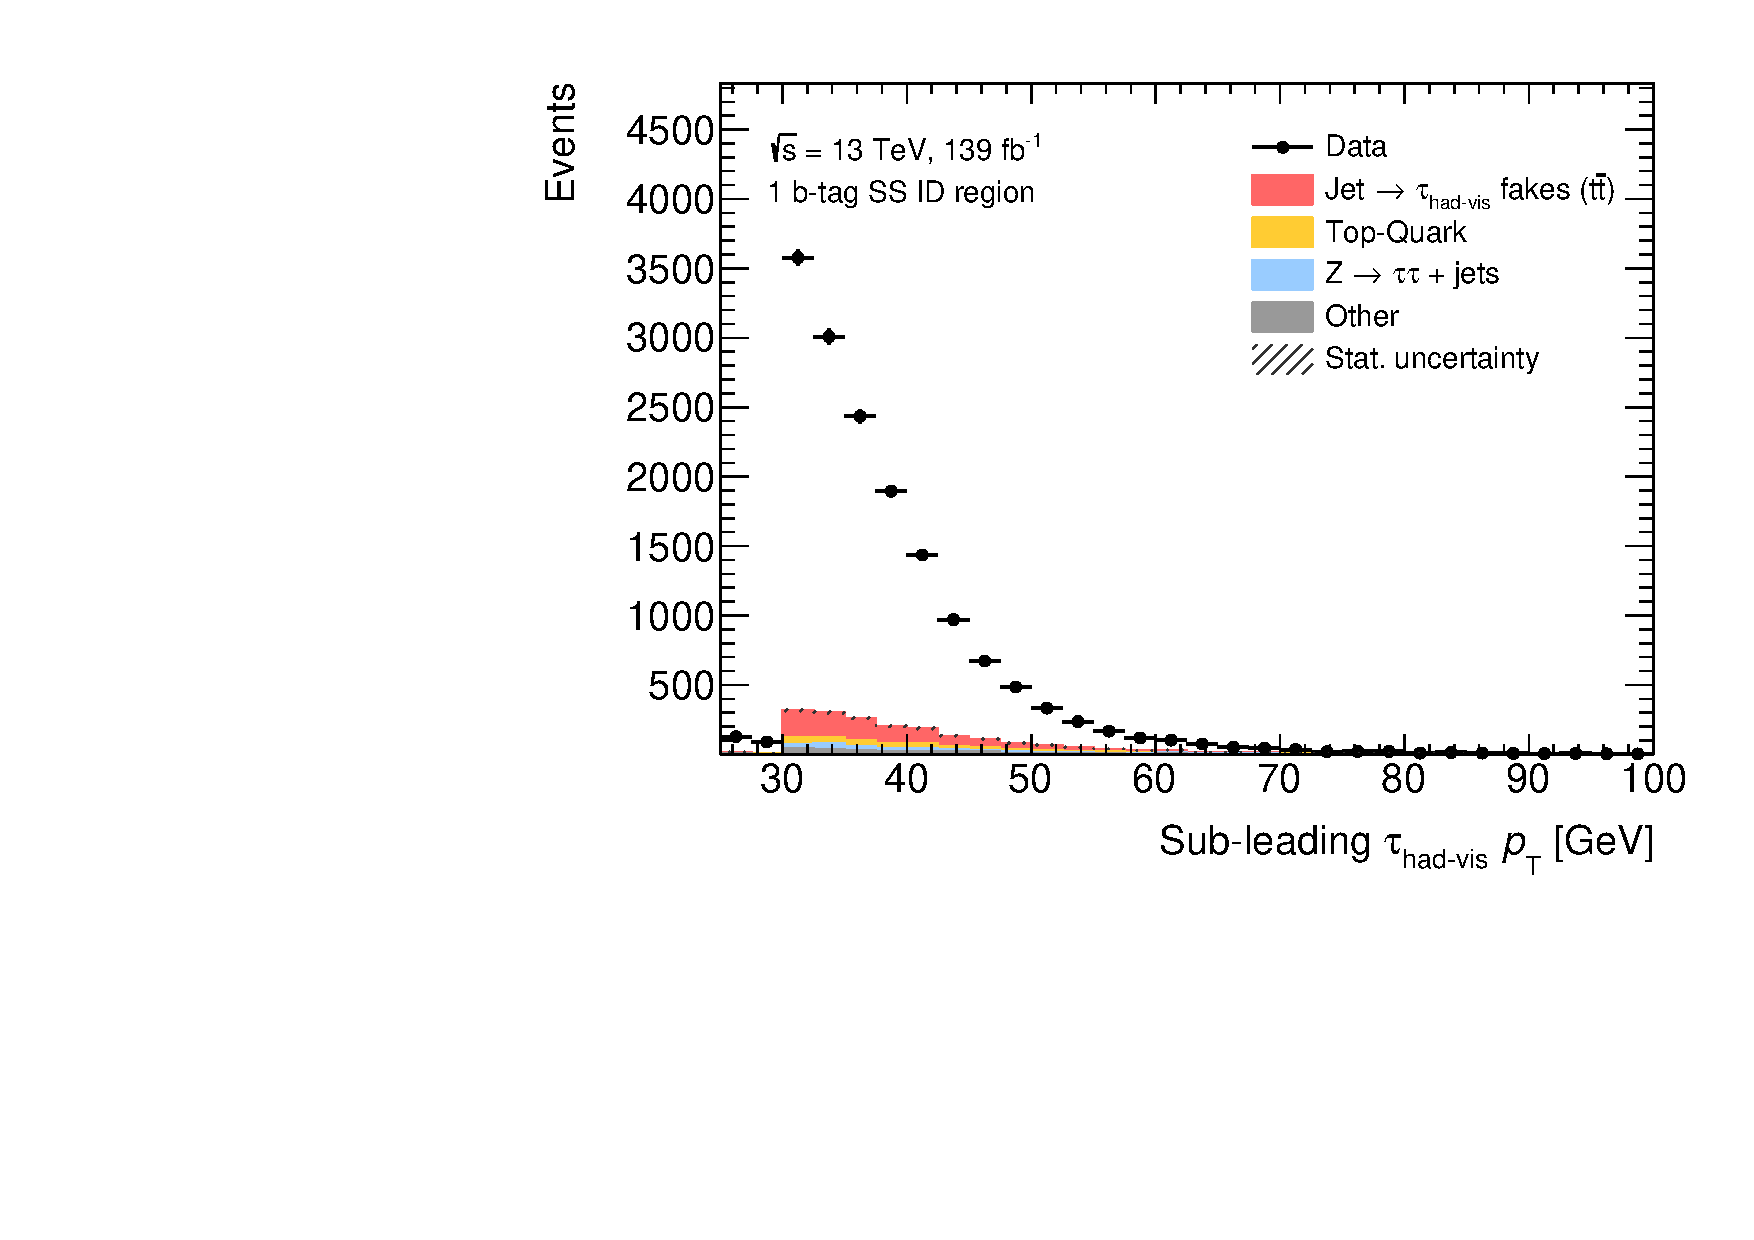
\includegraphics[width=\textwidth]{fakefactors/region_plots/tau1pt_1tag_ss_id}
    \subcaption{1 $b$-tag SS ID region}
  \end{subfigure}

  \begin{subfigure}{0.49\textwidth}
    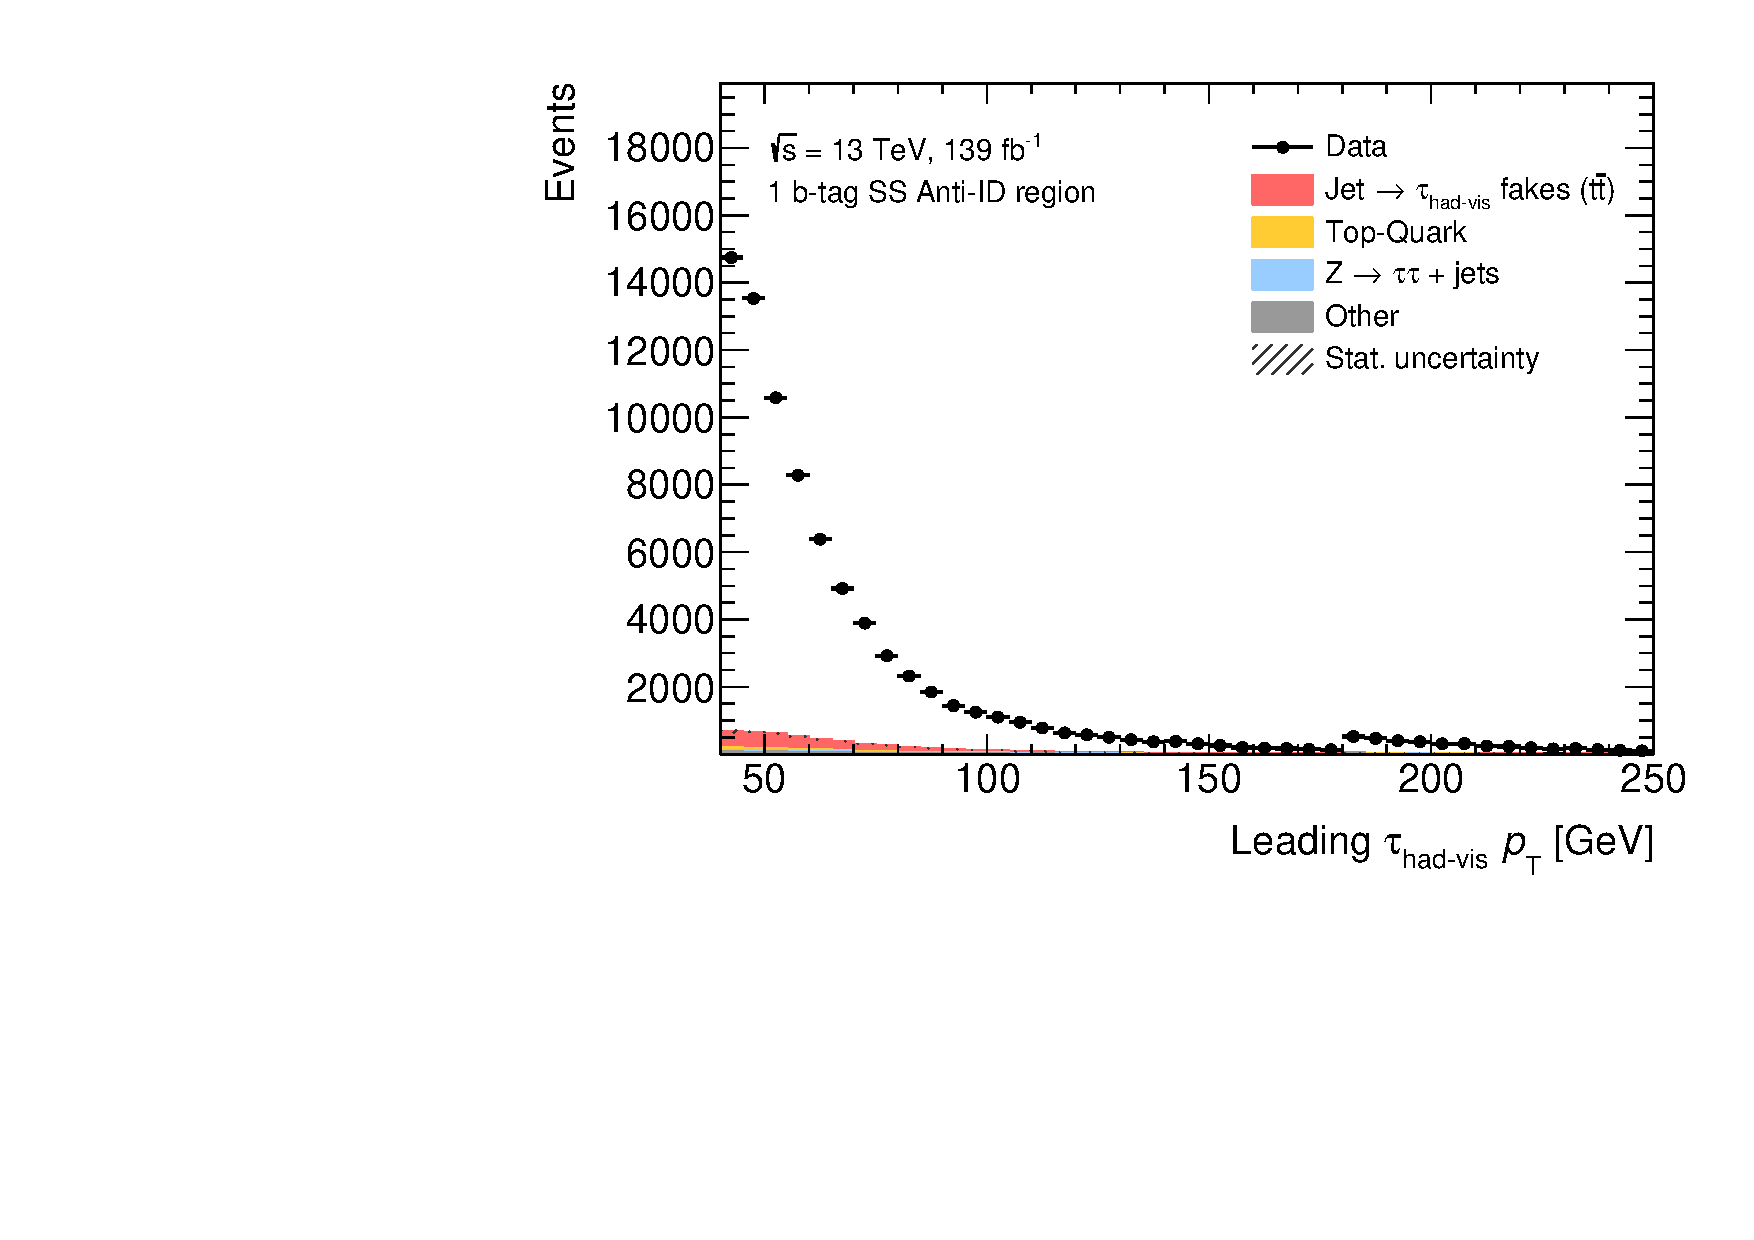
\includegraphics[width=\textwidth]{fakefactors/region_plots/tau0pt_1tag_ss_antiid}
    \subcaption{1 $b$-tag SS Anti-ID region}
  \end{subfigure}
  \begin{subfigure}{0.49\textwidth}
    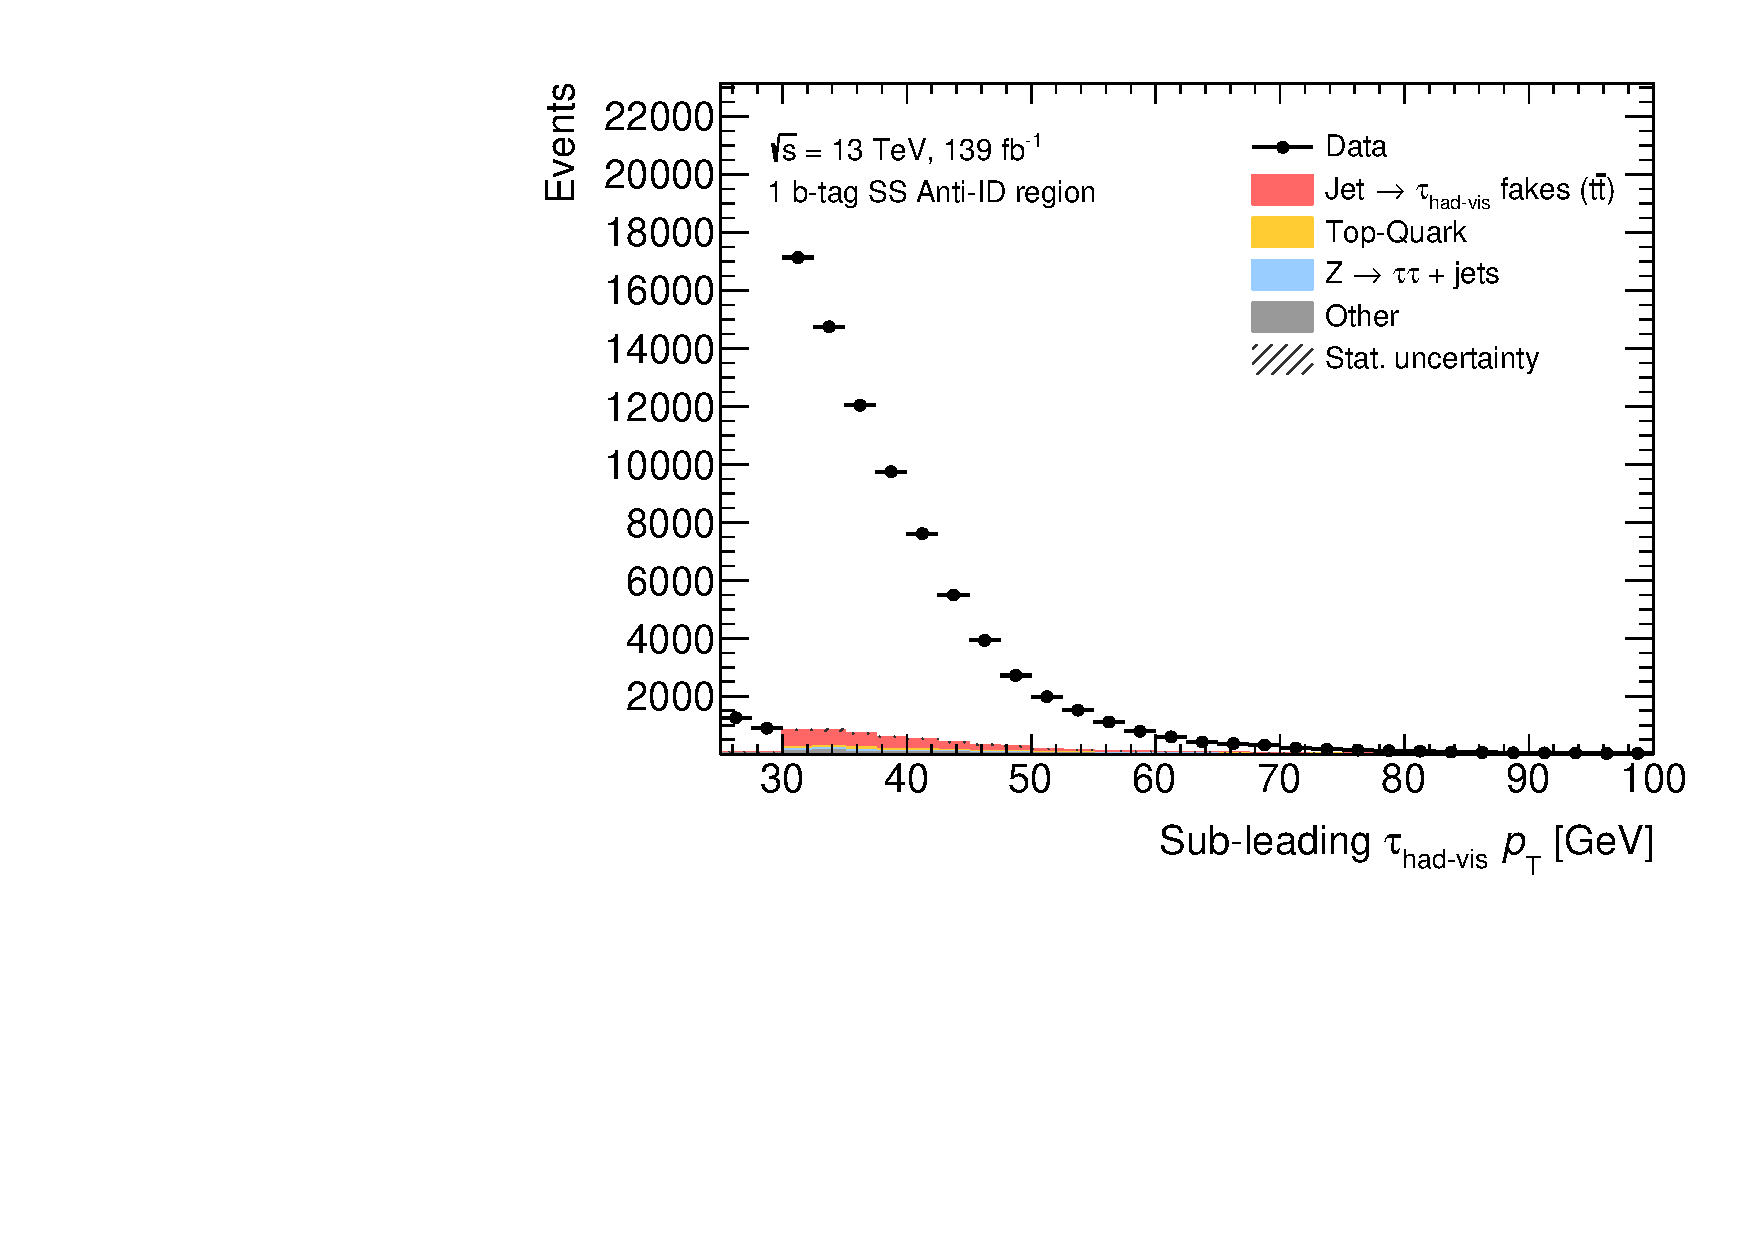
\includegraphics[width=\textwidth]{fakefactors/region_plots/tau1pt_1tag_ss_antiid}
    \subcaption{1 $b$-tag SS Anti-ID region}
  \end{subfigure}

  \caption{Distribution of leading and sub-leading \tauhadvis \pT for
    observed data and non-multi-jet backgrounds in regions entering
    the fake factor measurement. The 1 $b$-tag SS ID region is shown
    in (a,b) and the 1 $b$-tag SS Anti-ID region in (c,d). Coloured
    histograms depict the contributions of non-multi-jet processes
    that are subtracted during the fake factor measurement. The
    difference between the observed data and the non-multi-jet
    background estimate is attributed to the missing multi-jet
    background estimate. All regions are shown at pre-selection level
    corresponding to the SS region yields and multi-jet purities
    listed in~\Cref{tab:mjfakes_yields_1tag}.}%
  \label{fig:mjfakes_1tag_ss_plots}
\end{figure}

A schematic illustration of the approach is givens
in~\Cref{fig:fakefactor_regions}. Fake factors measured in the 1
$b$-tag regions ($\text{FF}_\text{SS}^\text{1-tag}$) are applied to
events in the 2 $b$-tag OS Anti-ID region after subtraction of
non-multi-jet contributions to obtain an estimate of the multi-jet
background in the signal region. Multiplicative transfer factors
($\text{TF}_{1 \ra 2\,b\text{-tag}}$) are applied to
$\text{FF}_\text{SS}^\text{1-tag}$ when used in 2 $b$-tag regions,
absorbing possible differences between fake factors measured in 1 and
2 $b$-tag regions and the uncertainties associated with this
extrapolation.

\begin{figure}[htbp]
  \centering

  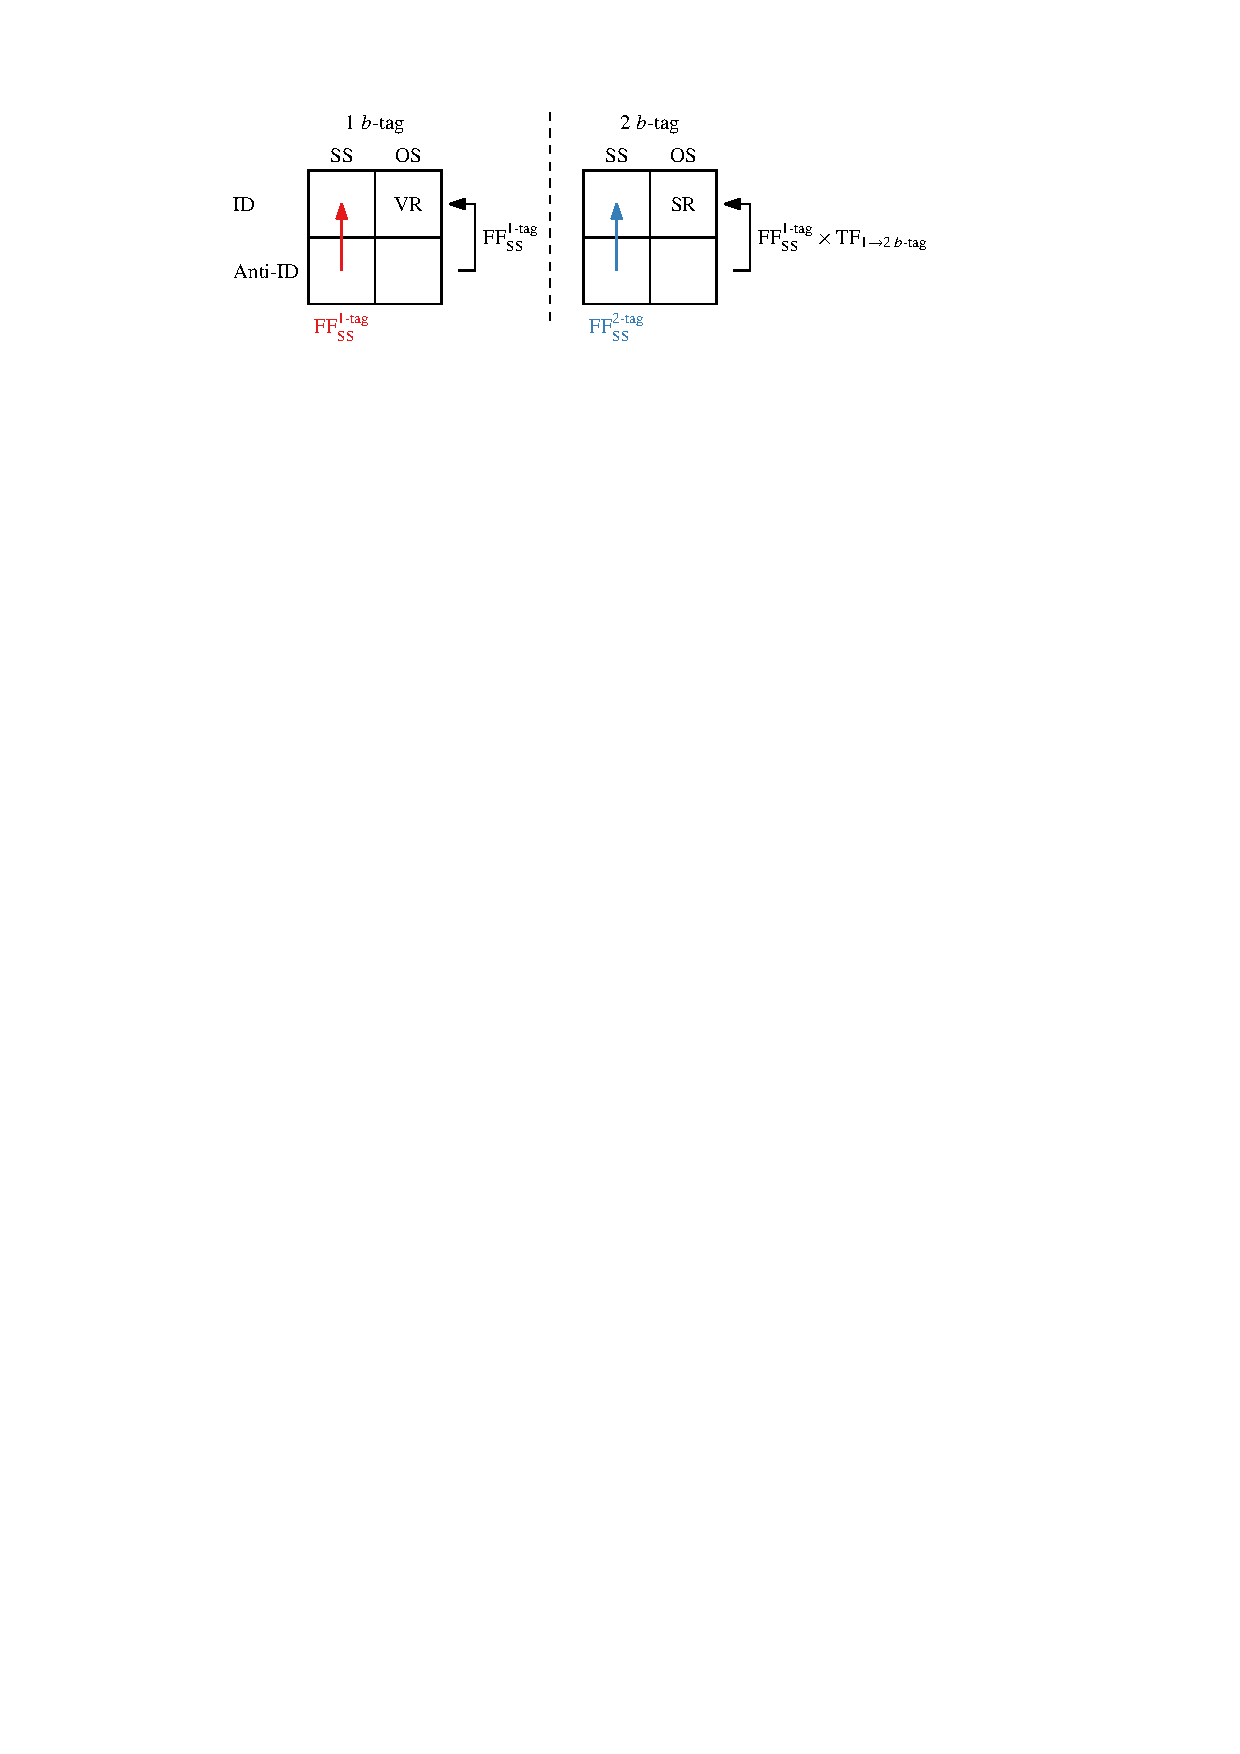
\includegraphics[scale=1]{fakefactors/regions}

  \caption{Schematic description of the fake factor method employed to
    estimate the multi-jet background in the signal region of the
    \hadhad channel. The squares represent the multi-jet events
    ($N_\text{multi-jet} = N_\text{data} - N_\text{non-multi-jet}$) in
    a particular region. The coloured arrows correspond to fake
    factors calculated as the ratio of multi-jet events in ID and
    Anti-ID regions.}
  \label{fig:fakefactor_regions}
\end{figure}

The 1 $b$-tag OS ID region serves as a validation region to check the
agreement of the total background prediction with the observed
data. Any non-closure observed in this region indicates either a
violation of the assumptions of the fake factor method, or a
parametrisation of the fake factors that is insufficient for the
modelling of the multi-jet background.

% % verify the independence of the observables related to \tauid and
% % electric charge of the \tauhadvis pair.
% This approach is equivalent to a comparison of fake factors measured
% in the OS and SS regions\footnote{\Cref{tab:mjfakes_yields_1tag} can
%   be used to calculate inclusive fake factors in the OS and SS
%   regions, yielding
%   $\text{FF}_\text{SS}^\text{1-tag} \approx
%   \text{FF}_\text{OS}^\text{1-tag} \approx 0.18$, which is a
%   sufficient condition for statistical independence of the fake factor
%   observables at the level of the inclusive selection.}, which have to
% agree under the assumptions of the method.\todo{Needs some work...}


\subsubsection{Measurement of fake factors}

% Binning in years / trigger
The fake factor measurement is performed separately for events
selected by single- and di-\tauhadvis triggers as well as the years of
data collection. During Run~2 of the LHC different \tauhadvis trigger
chains were used by the ATLAS experiment to collect the data used in
this analysis. As a result, the topologies of selected events and the
\tauid applied at the high-level trigger changed as Run~2
progressed. To account for possible differences resulting from the
change in trigger-selection, the fake factor measurement is performed
separately for three major data collection periods: 2015-2016, 2017,
and 2018.
% The 1 $b$-tag SS regions relevant to the measurement of fake factors
% are shown in~\Cref{fig:mjfakes_1tag_ss_plots}.

% Reason for binning in
The categorisation of the fake factors by trigger that selected the
event is further motivated by the differences between single- and
di-\tauhadvis triggers. Single-\tauhadvis triggers require one
\tauhadvis candidate with high transverse momentum that is identified
at the HLT without any selections applied to the other candidate. In
contrast, di-\tauhadvis triggers require two \tauhadvis to be
identified at the HLT with similar transverse momentum thresholds
applied to both. This allows \tauhadvis candidates in in the
di-\tauhadvis trigger category to be treated equally once
\pT-threshold effects are accounted for. This is not the case for
events selected by single-\tauhadvis triggers.

Dependencies of the fake factors on reconstructed quantities of
\tauhadvis candidates are accounted for by further categorisation
based on properties of the \tauhadvis that distinguishes the ID from
the Anti-ID regions. The fake factor measurement is performed
separately for 1- and 3-prong \tauhadvis candidates for both trigger
categories.

Fake factors for events selected by di-\tauhadvis triggers are
additionally measured in bins of \tauhadvis~\pT and separately for
\tauhadvis in the barrel and endcap regions of the ATLAS detector.

In contrast, few multi-jet events enter the single-\tauhadvis trigger
category due to large \pT thresholds on the leading \tauhadvis. This
prevents a further subdivision of the fake factor measurement in this
category into many bins. Therefore, the fake factors for
singe-\tauhadvis trigger events are measured separately for cases
where the anti-\tauhadvis is leading and the sub-leading in \pT. This
accounts for differences in HLT \tauid and the typically large
differences in \pT between the leading and sub-leading
\tauhadvis~candidates.

\subsubsection{Measurement of fake factors: di-\tauhadvis triggers}

{% Group for extra definitions
  \newcommand*{\ffargs}{\ensuremath{( \myvec{x}_{\tau} )}\xspace}

  \newcommand*{\NmjID}[2]{\ensuremath{N_\text{multi-jet}^{\text{#1, loose }\tau_{#2}}}\xspace}
  \newcommand*{\NmjIDIncl}[1]{\ensuremath{N_\text{multi-jet}^{\text{#1, ID}}}\xspace}

  \newcommand*{\NmjAntiIDIncl}[1]{\ensuremath{N_\text{multi-jet}^{\text{#1, Anti-ID}}}\xspace}
  \newcommand*{\NmjAntiID}[2]{\ensuremath{N_\text{multi-jet}^{\text{#1, anti-}\tau_{#2}}}\xspace}

  The Anti-ID region can be partitioned into two sub-regions: one
  where the anti-\tauhadvis is the leading and one where it is the
  sub-leading \tauhadvis candidate. Provided the conditions for the
  fake factor method are fulfilled, both regions can be used to obtain
  separate estimates of the multi-jet background in the OS ID
  region. The notation used to describe the fake factor measurement is
  introduced in the following:
  \begin{description}[style=standard]
  \item[$\tau_0$ ($\tau_1$)] The \tauhadvis candidate leading (sub-leading) in \pT.

  \item[$\myvec{x}_\tau$] A vector of categorical observables related
    to a \tauhadvis that defines the bin of the fake factor
    measurement. The measurement in the di-\tauhadvis trigger category
    is performed separately for 1- and 3-prong \tauhadvis, and in bins
    of \tauhadvis \pT and $\eta$.

  \item[$\NmjID{SS(OS)}{i}\ffargs$] The estimated number of multi-jet
    events in the SS (OS) ID region where~$\tau_i$ has
    observables~$\myvec{x}_\tau$.

  \item[$\NmjAntiID{SS(OS)}{i}\ffargs$] The estimated number of
    multi-jet events in the SS (OS) Anti-ID region where $\tau_i$ is
    the anti-\tauhadvis with observables~$\myvec{x}_\tau$.
  \end{description}
  With these definitions, two sets of fake factors can be defined as
  \begin{align*}
    \FF_{i}\ffargs &= \frac{\NmjID{SS}{i} \ffargs}{\NmjAntiID{SS}{i}\ffargs}
                     \quad \text{for} \quad i = 0, 1 \,\text{,}
  \end{align*}
  where $\FF_{i}$ is the fake factor relating the ID region with the
  partition of the Anti-ID region where $\tau_i$ is the
  anti-\tauhadvis. These can be used to obtain two multi-jet estimates
  in the OS region given by
  \begin{align*}
    \NmjID{OS}{i}\ffargs = \FF_{i}\ffargs \cdot \NmjAntiID{OS}{i}\ffargs
    \quad \text{for} \quad i = 0, 1 \,\text{.}
  \end{align*}
  An average of both estimates can be calculated, yielding fake
  factors that are inclusive in whether the anti-\tauhadvis is the
  leading or sub-leading \tauhadvis candidate. The inclusive fake
  factors can be expressed as
  \begin{align*}
    \FF_\text{incl.}\ffargs = \frac{1}{2} \left[ f_0\ffargs \cdot \FF_0\ffargs
    + f_1\ffargs \cdot \FF_1\ffargs \right] \,\text{,}
  \end{align*}
  with $f_i\ffargs$ being the fraction of Anti-ID events where
  $\tau_i$ is the anti-\tauhadvis for a given bin $\myvec{x}_\tau$ of
  the anti-\tauhadvis:
  \begin{align*}
    f_i\ffargs = \frac{\NmjAntiID{SS}{i}\ffargs}
                      {\NmjAntiID{SS}{0}\ffargs + \NmjAntiID{SS}{1}\ffargs} \,\text{.}
  \end{align*}
  The inclusive fake factor can be measured directly according to
  \begin{align}
    \FF_\text{incl.}\ffargs
    = \frac{1}{2} \frac{ \NmjID{SS}{0}\ffargs + \NmjID{SS}{1}\ffargs }
                       { \NmjAntiID{SS}{0}\ffargs + \NmjAntiID{SS}{1}\ffargs }
    \label{eq:inclusive_fake_factor}
  \end{align}
  and the multi-jet estimate in the OS region obtained by\todo{Should there be a $\sum_{x_\tau}$ here?}
  \begin{align*}
    \NmjIDIncl{OS}\ffargs = \FF_\text{incl.}\ffargs \cdot \NmjAntiIDIncl{OS}\ffargs \,\text{,}
  \end{align*}
  where $\NmjAntiIDIncl{OS}\ffargs$ is the number of multi-jet events
  in the inclusive OS Anti-ID region with anti-\tauhadvis in the bin
  given by~$\myvec{x}_\tau$.

  % Prior the agreement of the background estimates obtained with FF0
  % and FF1 were confirmed.

  The motivation of using inclusive fake factors is two-fold. First,
  it allows to use all events entering the Anti-ID region, independent
  of whether the anti-\tauhadvis is leading or sub-leading in \pT,
  thus improving the statistical precision of the background
  estimate. Second, the fake factors can be parametrised in the
  properties of the anti-\tauhadvis directly, allowing to target the
  key differences between the ID and Anti-ID regions. This represents
  a change with respect to the previous
  publication~\cite{HIGG-2016-16-witherratum} where fake factors were
  parametrised jointly in the properties of both \tauhadvis
  candidates, thus limiting the statistical precision of the fake
  factor measurement due to high dimensionality.
}

The inclusive fake factors for events selected by di-\tauhadvis
triggers are measured according to~\Cref{eq:inclusive_fake_factor} and
parametrised in \tauhadvis decay mode, transverse momentum,
pseudorapidity, and the period of data collection. The number of
multi-jet events is obtained by subtracting the expected number of
non-multi-jet events estimated using simulation from the number of
observed events in data.

The result of the fake factor measurement is summarised
in~\Cref{fig:mjfakes_fake_factors}. Qualitatively, the behaviour of
the fake factors with respect to the \tauhadvis properties is the same
between all data collection periods. Minor differences exist when
comparing different data-taking periods. No attempt was made to
combine the measurements of certain periods as the statistical
precision of the fake factor measurement is not a limiting factor in
the analysis.

\begin{figure}[htbp]
  \centering

  \begin{subfigure}{0.495\textwidth}
    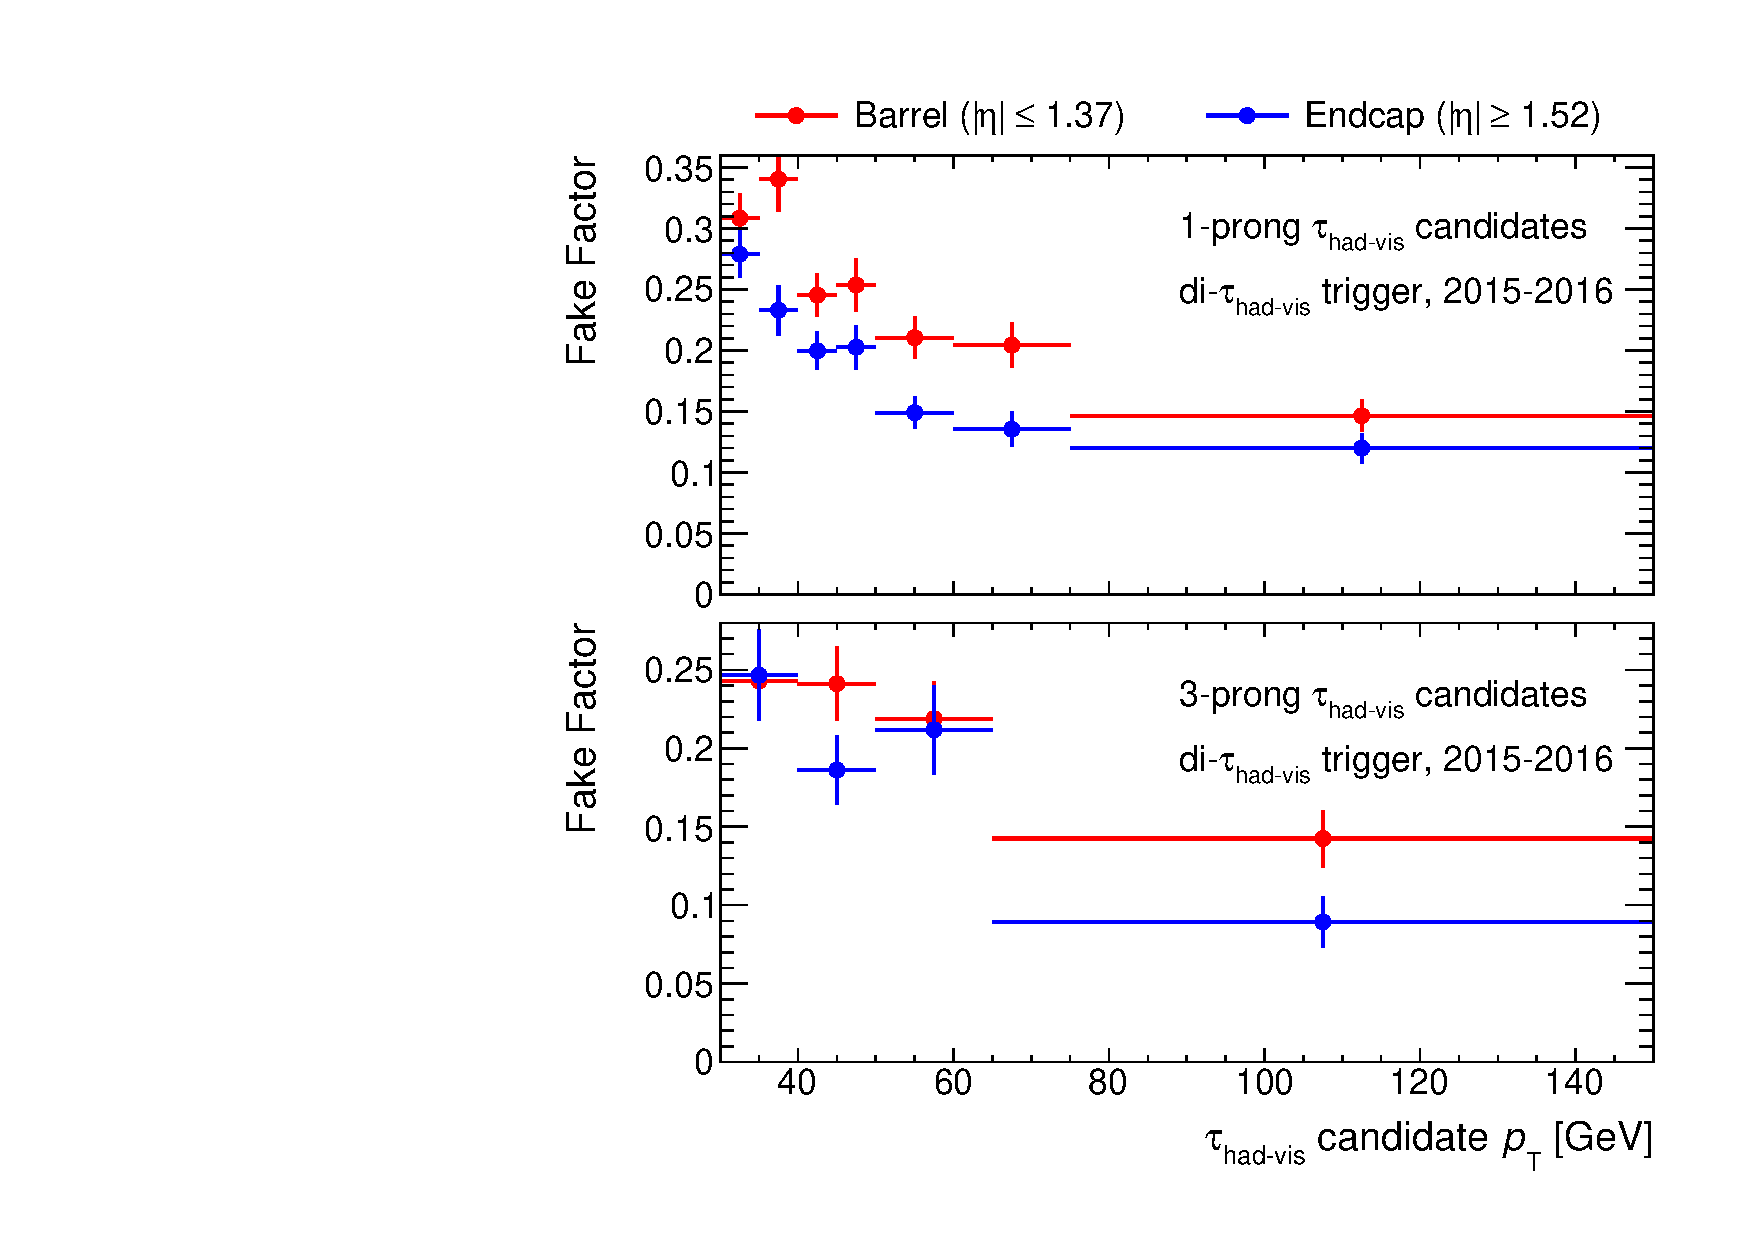
\includegraphics[width=\textwidth]{fakefactors/fake_factors_dtt_1516}
    \subcaption{2015-2016 data collection period}
  \end{subfigure}
  \begin{subfigure}{0.495\textwidth}
    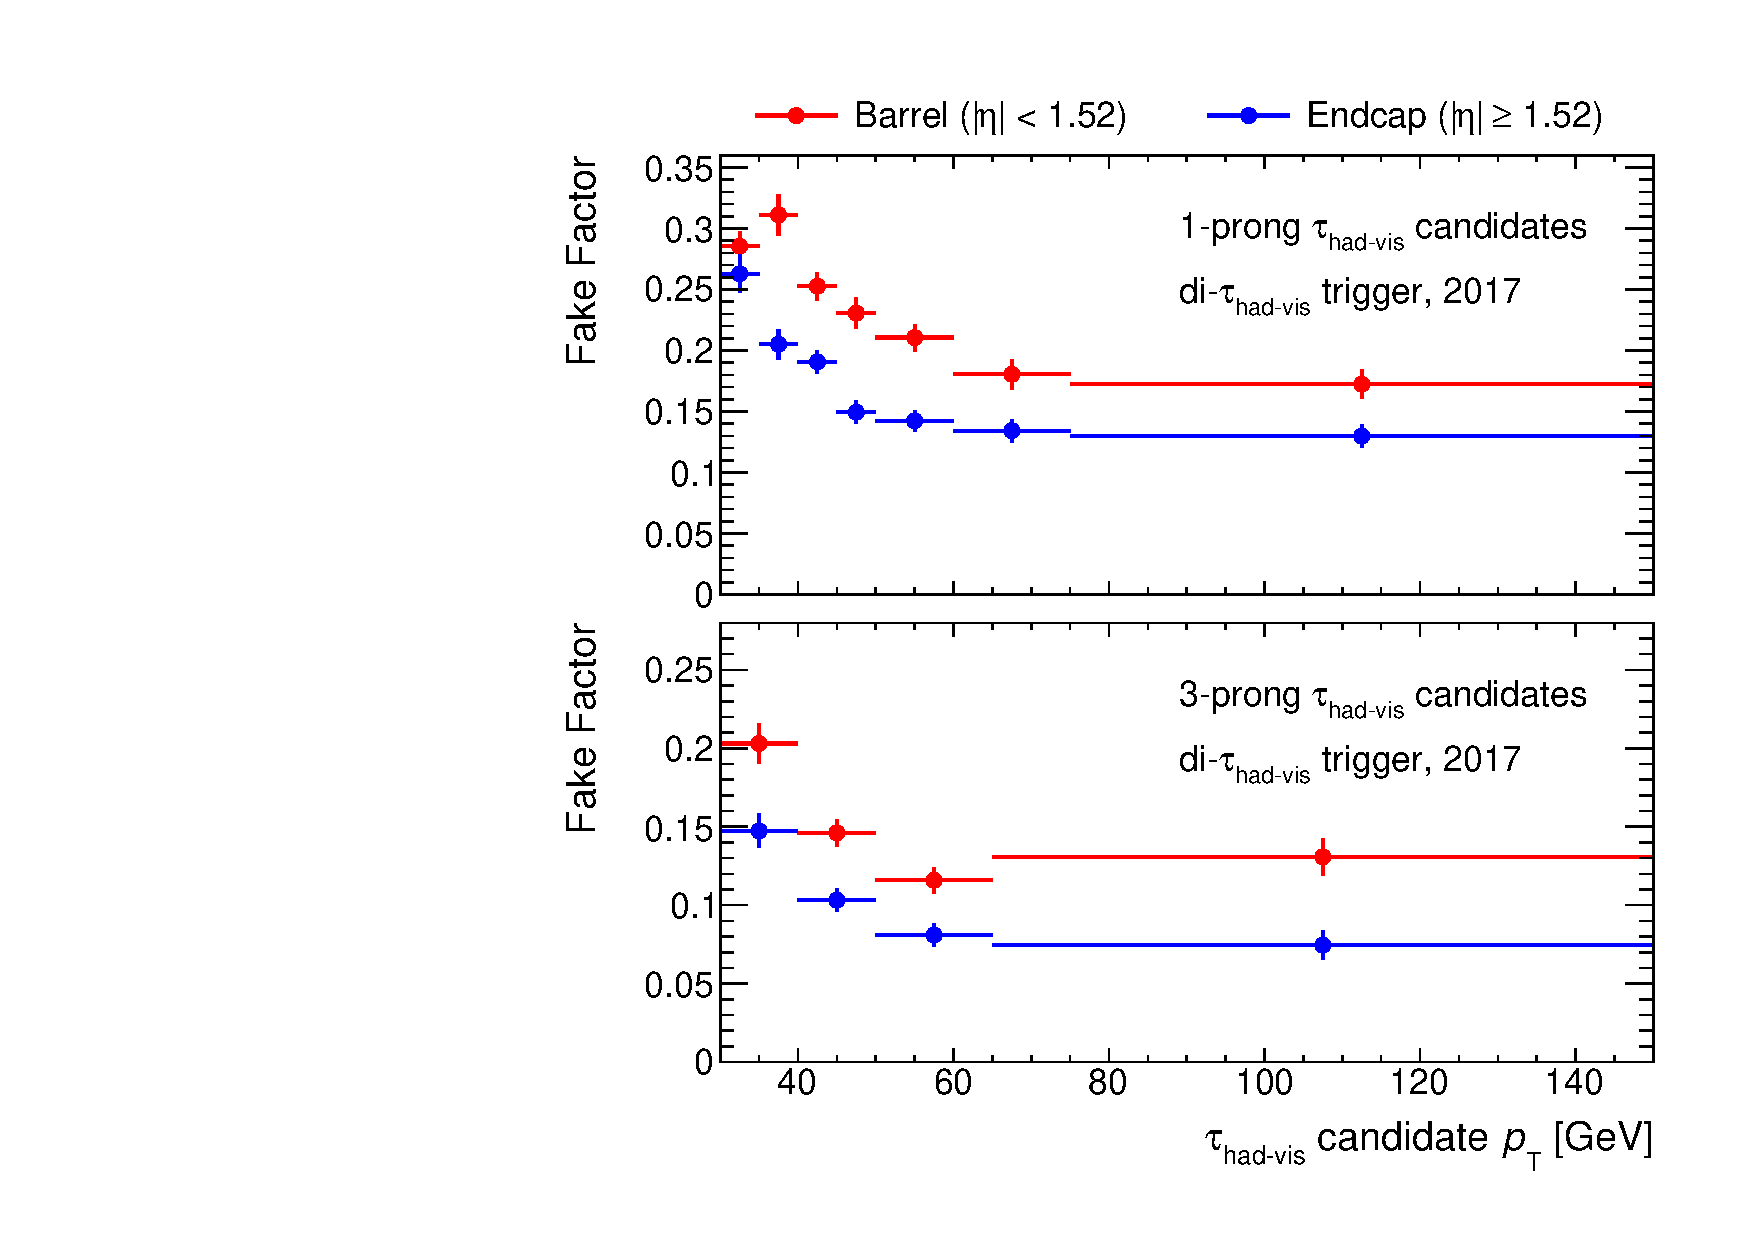
\includegraphics[width=\textwidth]{fakefactors/fake_factors_dtt_17}
    \subcaption{2017 data collection period}
  \end{subfigure}

  \begin{subfigure}{0.495\textwidth}
    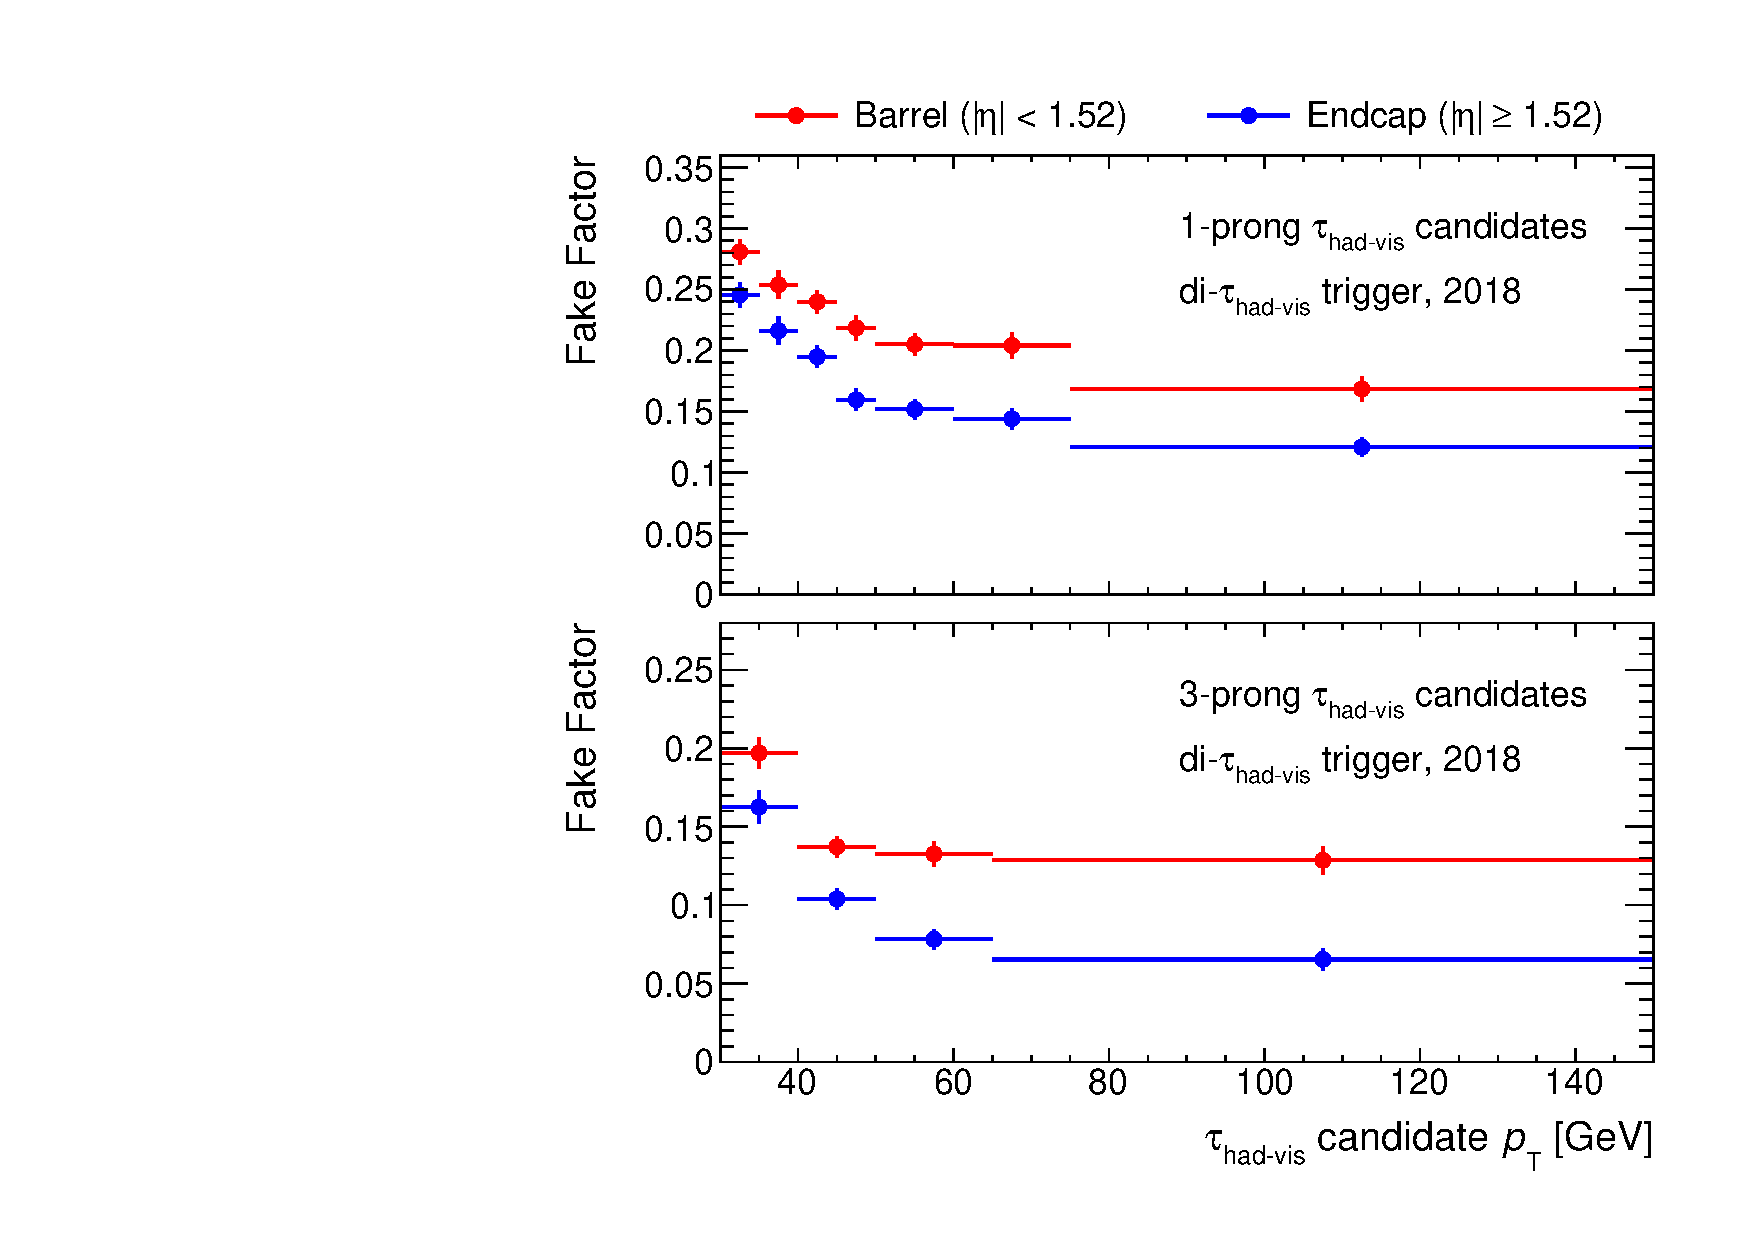
\includegraphics[width=\textwidth]{fakefactors/fake_factors_dtt_18}
    \subcaption{2018 data collection period}
  \end{subfigure}

  \caption{Inclusive fake factors for events selected by di-\tauhadvis
    triggers measured in the 1 $b$-tag SS region. The measurement is
    performed separately for the three major data collection periods
    (a-c), 1- and 3-prong \tauhadvis candidates (upper / lower
    panels), and for \tauhadvis in the barrel (red) and endcap regions
    (blue) of the ATLAS detector. Events with (anti-)\tauhadvis
    $\pT > \SI{150}{\GeV}$ are included in the last fake factor
    bin. Uncertainties are from statistical sources only. Systematic
    uncertainties originating from the non-multi-jet subtraction are
    assumed to be negligible due to the small size of the subtraction
    in the 1 $b$-tag SS region.}
  \label{fig:mjfakes_fake_factors}
\end{figure}


\subsubsection{Measurement of fake factors: single-\tauhadvis
  triggers}

The measurement of fake factors for events selected by
single-\tauhadvis triggers has to proceed differenty from the
di-\tauhadvis trigger case. First, at the HLT \tauhadvis
identification is only applied to one of the \tauhadvis candidates,
preventing an inclusive treatment of both \tauhadvis
candidates. Second, the high \pT thresholds on \tauhadvis at
trigger-level has high rejection of most SM processes, limiting the
number of events entering the control regions for the fake factor
measurement. As a result, the fake factors for singe-\tauhadvis
triggers cannot be measured differentially in \tauhadvis \pT and
$\eta$.

\todo[inline]{FIXME}

The STT fake factors are measured in four categories for every major
period of data collection: 1- and 3-prong \tauhadvis and whether the
\tauhadvis is leading or sub-leading in \pT. The resulting fake
factors are summarised in~\Cref{fig:mjfakes_stt_ffs}.

\begin{figure}[htbp]
  \centering

  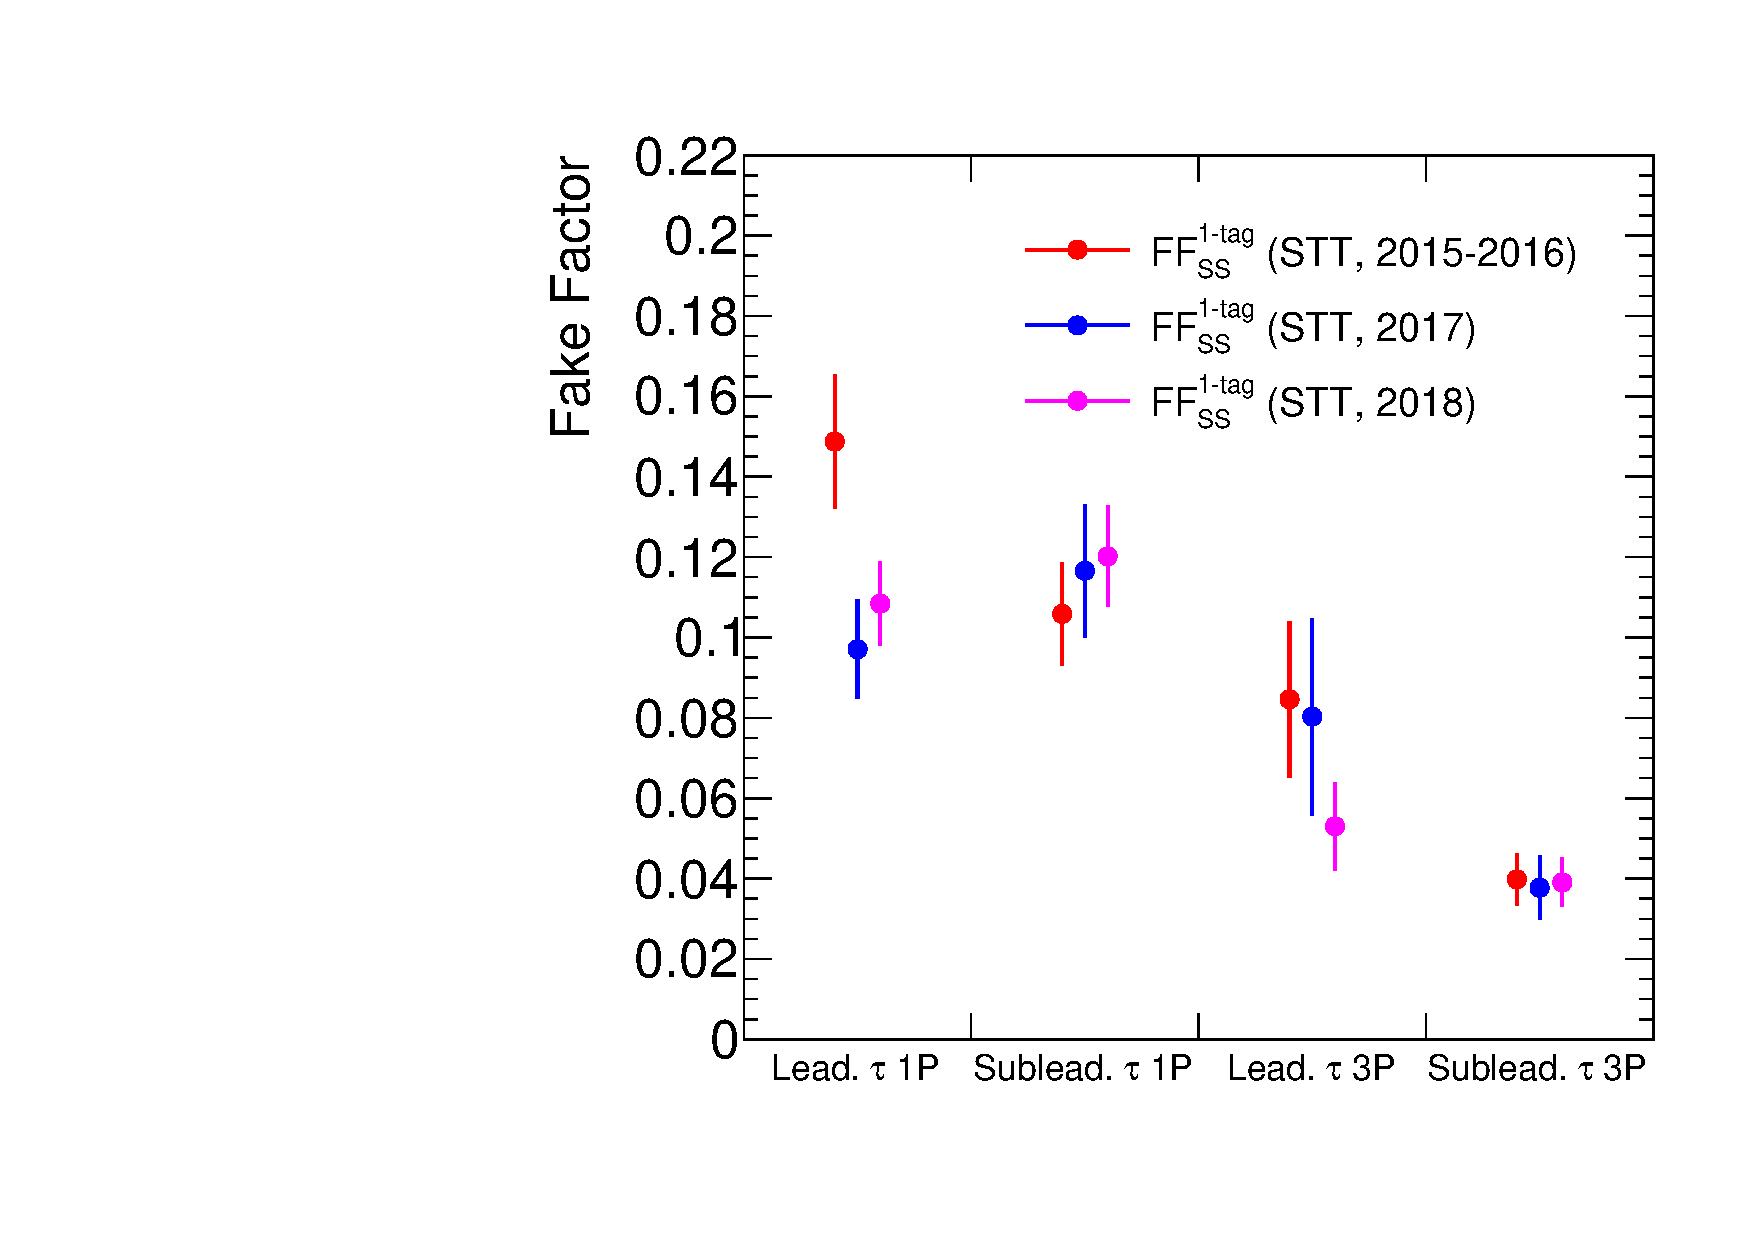
\includegraphics[width=0.495\textwidth]{fakefactors/fake_factors_stt}

  \caption{Fake factors (1 $b$-tag SS) for events selected by
    single-\tauhadvis triggers measured separately for the three major
    data collection periods. The measurement is performed (inclusively
    in \tauhadvis \pT and $\eta$) in bins of the reconstructed
    \tauhadvis decay mode (1- and 3-prong) and separately for cases
    where the \pT leading and sub-leading \tauhadvis is the
    anti-\tauhadvis ($\tau_0$ and $\tau_1$).}%
  \label{fig:mjfakes_stt_ffs}

  \todo[inline]{Largest deviation for leading 1-prong tau possibly due
    to looser pT threshold.}
\end{figure}


\subsubsection{Validation of the Fake Estimate in 1 $b$-tag OS}

An independent validation of the background estimation technique can
be performed in the 1 $b$-tag OS region, which is not part of the fake
factor measurement. At pre-selection level, this region has a
multi-jet purity of about \SI{50}{\percent} with other contributions
from $\Zjets$ and \ttbar. The multi-jet purity can be increased for
validation purposes of the multi-jet background estimate by requiring
% https://twiki.cern.ch/twiki/bin/view/AtlasProtected/MetSignificance
% Using `TreatPUJets == true' and Basic soft term (met::Random)
\begin{align*}
  \mMMC > \SI{110}{\GeV} \qquad \text{and} \qquad \mathcal{S} < 3 \,\text{,}
\end{align*}
where $\mathcal{S}$ is the object-based \pTmissAbs
significance~\cite{ATLAS-CONF-2018-038} that measures the statistical
significance of a test probing the hypothesis of no real \pTmissAbs
compared to the alternative of having real \pTmissAbs. The
contribution of \Zjets is reduced by rejecting events close to the \PZ
boson mass. Multi-jet events are expected to have little real
\pTmissAbs, thus events with significant \pTmissAbs are rejected to
reduce the \ttbar contribution in this
region. In~\Cref{fig:fake_factor_OSVR_cutvars} both variables are
shown in the 1 $b$-tag OS region at pre-selection level to illustrate
this choice of selection for the multi-jet validation region. The
purity of multi-jet validation region is increased to about
\SI{75}{\percent}.

\begin{figure}[htbp]
  \centering

  \begin{subfigure}{0.45\textwidth}
    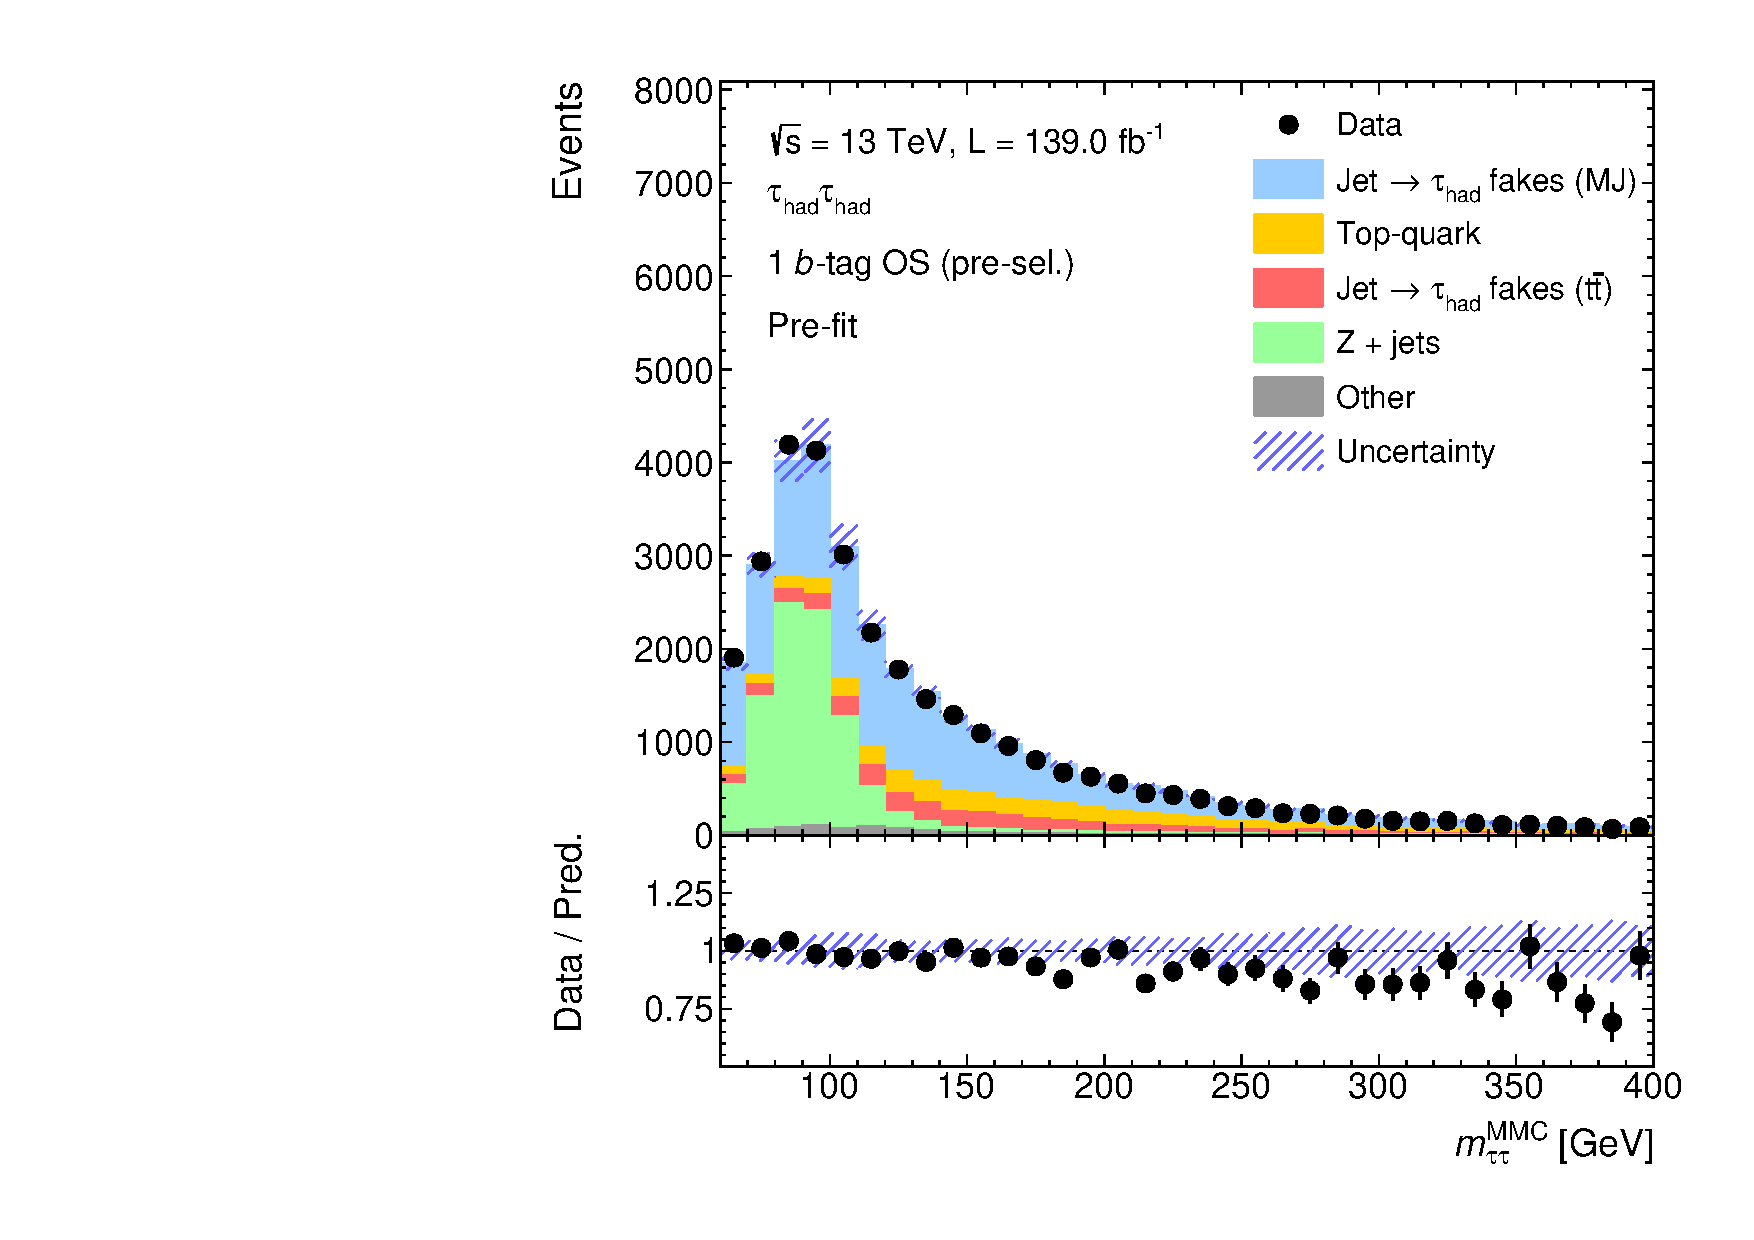
\includegraphics[width=\textwidth]{fakefactors/fake_os_vr/mMMC_presel}
    \subcaption{}
  \end{subfigure}\hspace*{0.04\textwidth}%
  \begin{subfigure}{0.45\textwidth}
    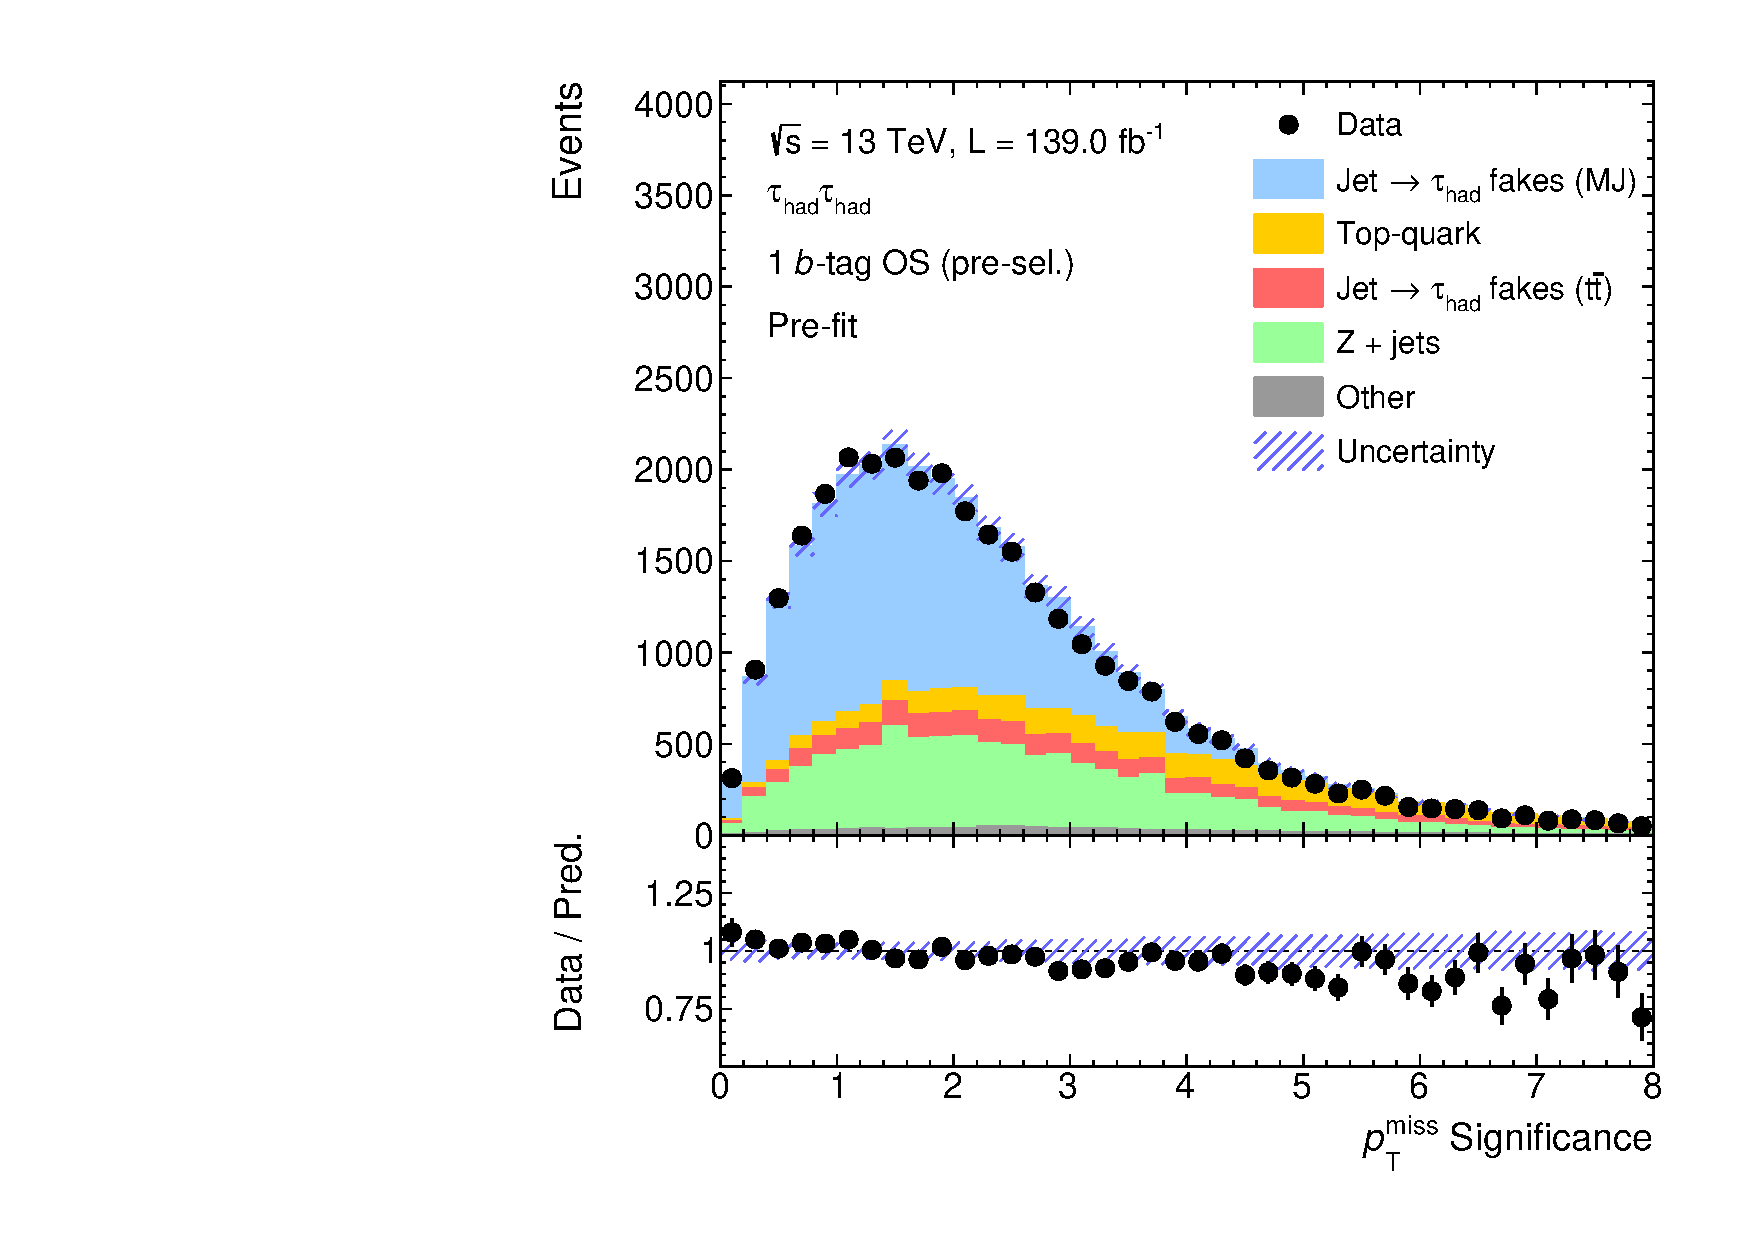
\includegraphics[width=\textwidth]{fakefactors/fake_os_vr/metSig_presel}
    \subcaption{}
  \end{subfigure}

  \caption{The invariant di-\tauhad mass (a) and the object-based
    \pTmissAbs significance (b) in the 1 $b$-tag OS ID region at
    pre-selection level. The estimate of the multi-jet background
    (light blue) is obtained using the fake factor method (cf.\
    \Cref{fig:fakefactor_regions}). Fake-\tauhadvis originating from
    \ttbar (red) are estimated using simulation. The background
    prediction is shown pre-fit, including statistical and
    detector-related systematic uncertainties.}
  \label{fig:fake_factor_OSVR_cutvars}
\end{figure}

The background prediction in the multi-jet validation region is
compared to data in~\Cref{fig:fake_factor_OSVR_kinematics}. The
multi-jet background is estimated using the fake factor method by
applying fake factors measured in the SS regions to events in the OS
Anti-ID region. The background prediction is in good agreement with
the observed data in the validation region, indicating the validity of
the assumptions made by the fake factor method.

\begin{figure}[p]
  \centering

  \begin{subfigure}{0.45\textwidth}
    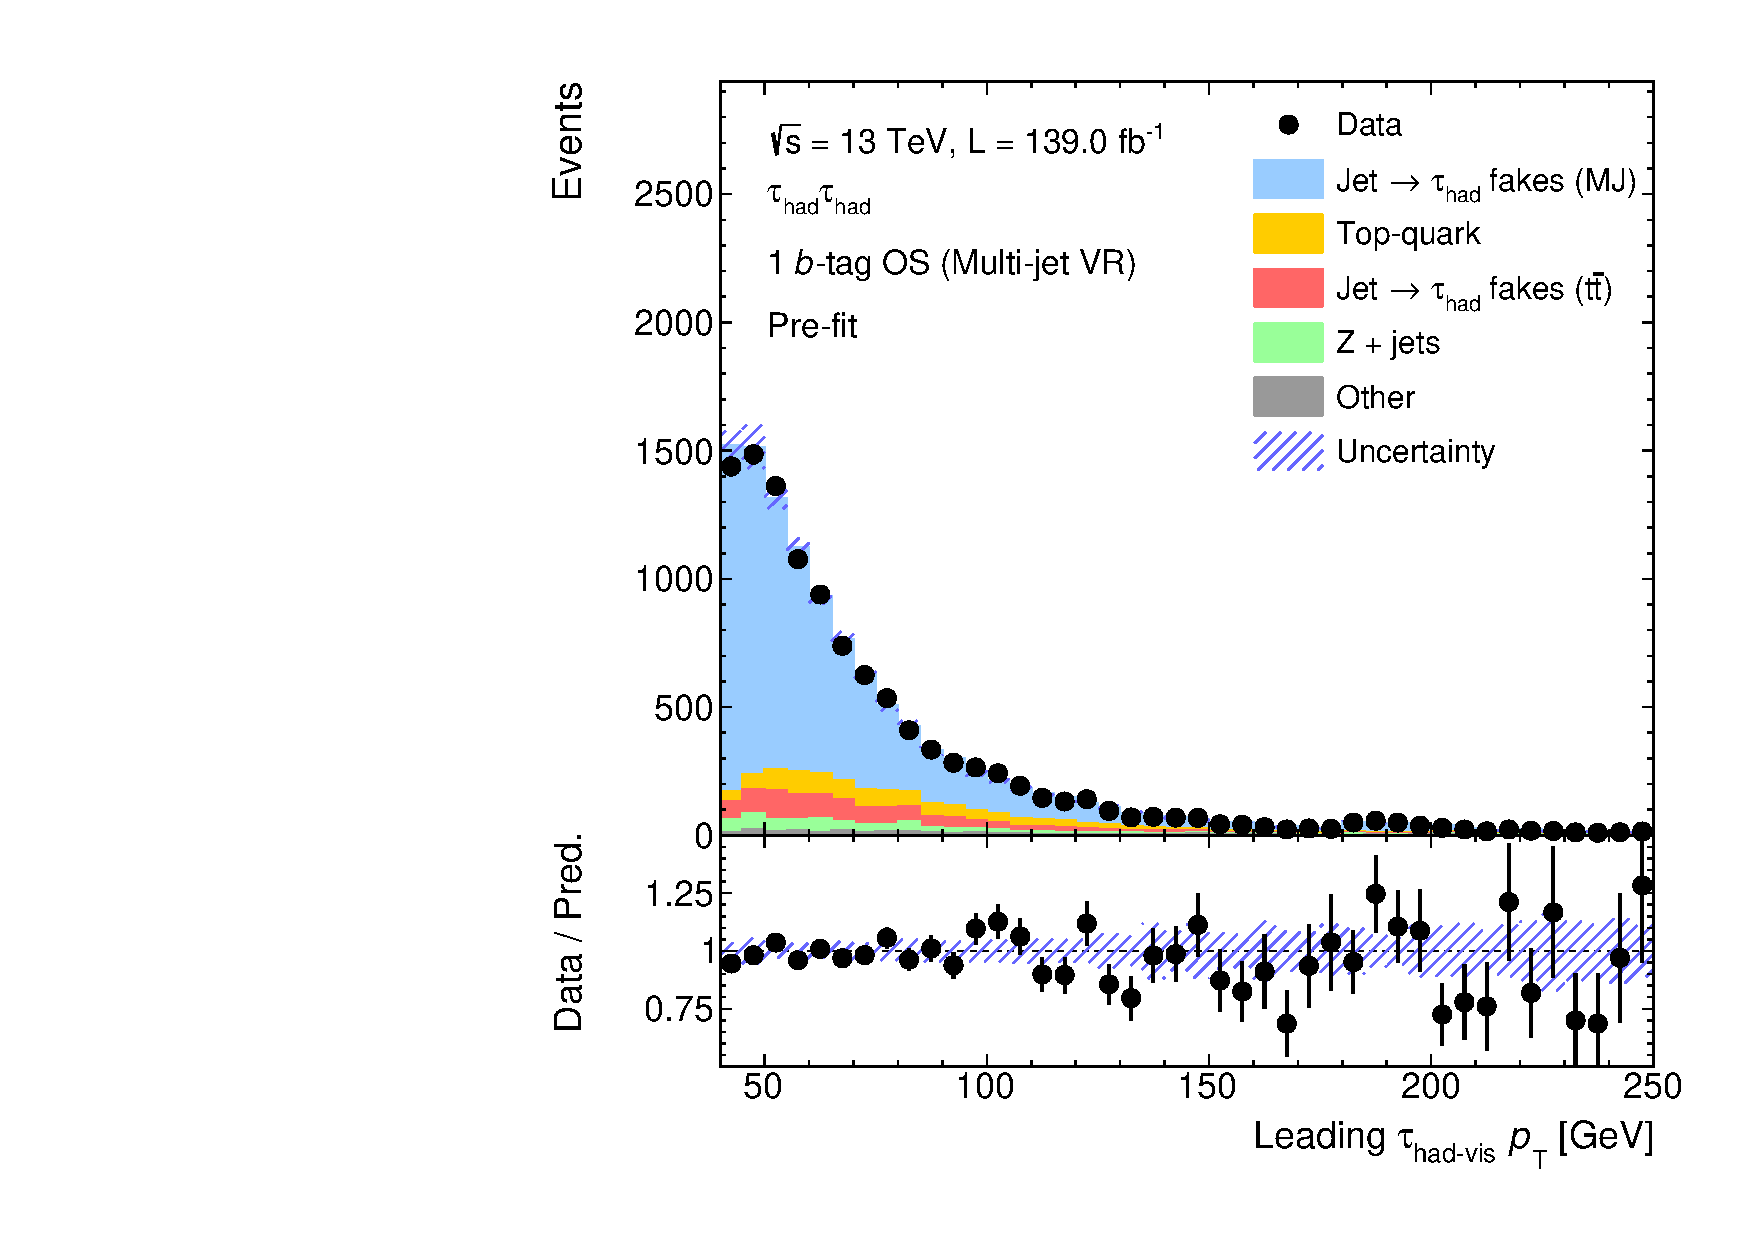
\includegraphics[width=\textwidth]{fakefactors/fake_os_vr/Tau0Pt_fakevr}
  \end{subfigure}\hspace*{0.04\textwidth}%
  \begin{subfigure}{0.45\textwidth}
    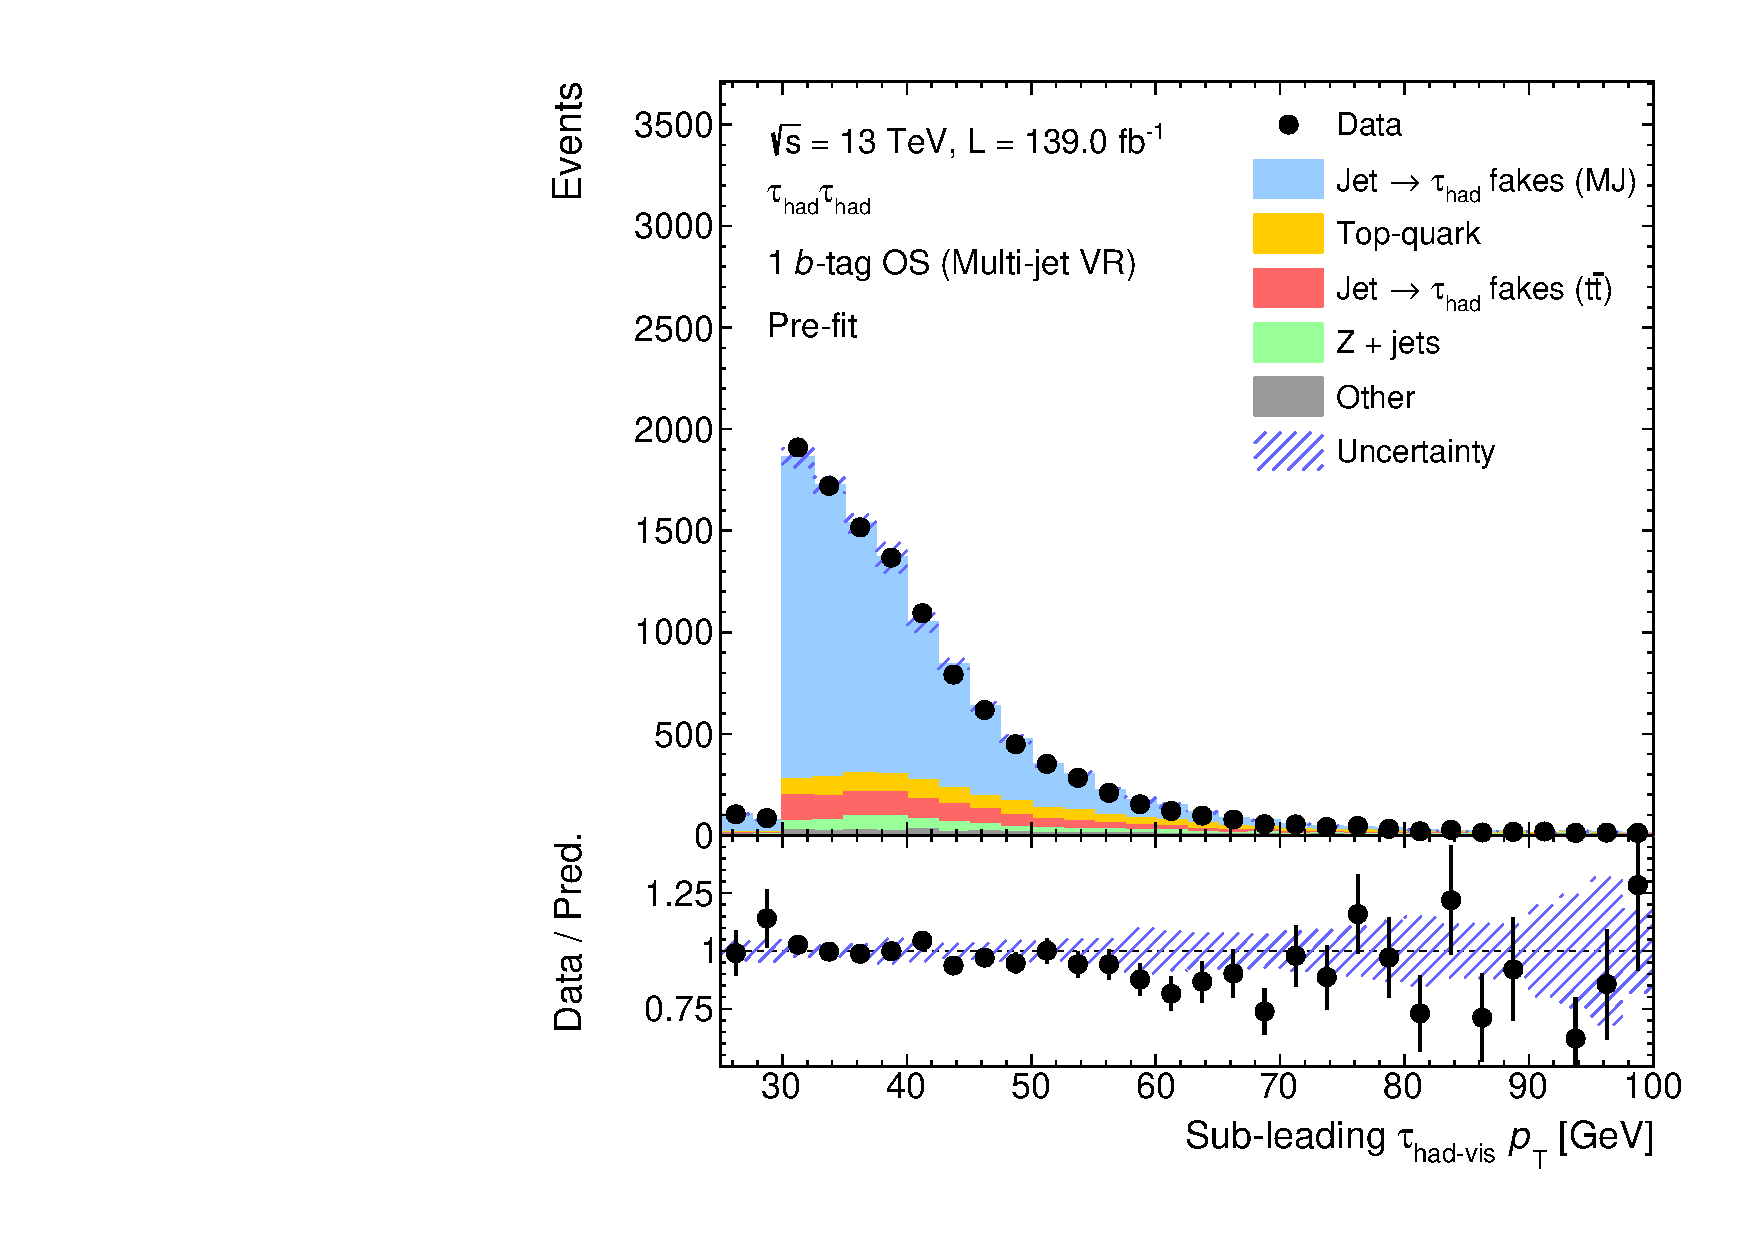
\includegraphics[width=\textwidth]{fakefactors/fake_os_vr/Tau1Pt_fakevr}
  \end{subfigure}

  \begin{subfigure}{0.45\textwidth}
    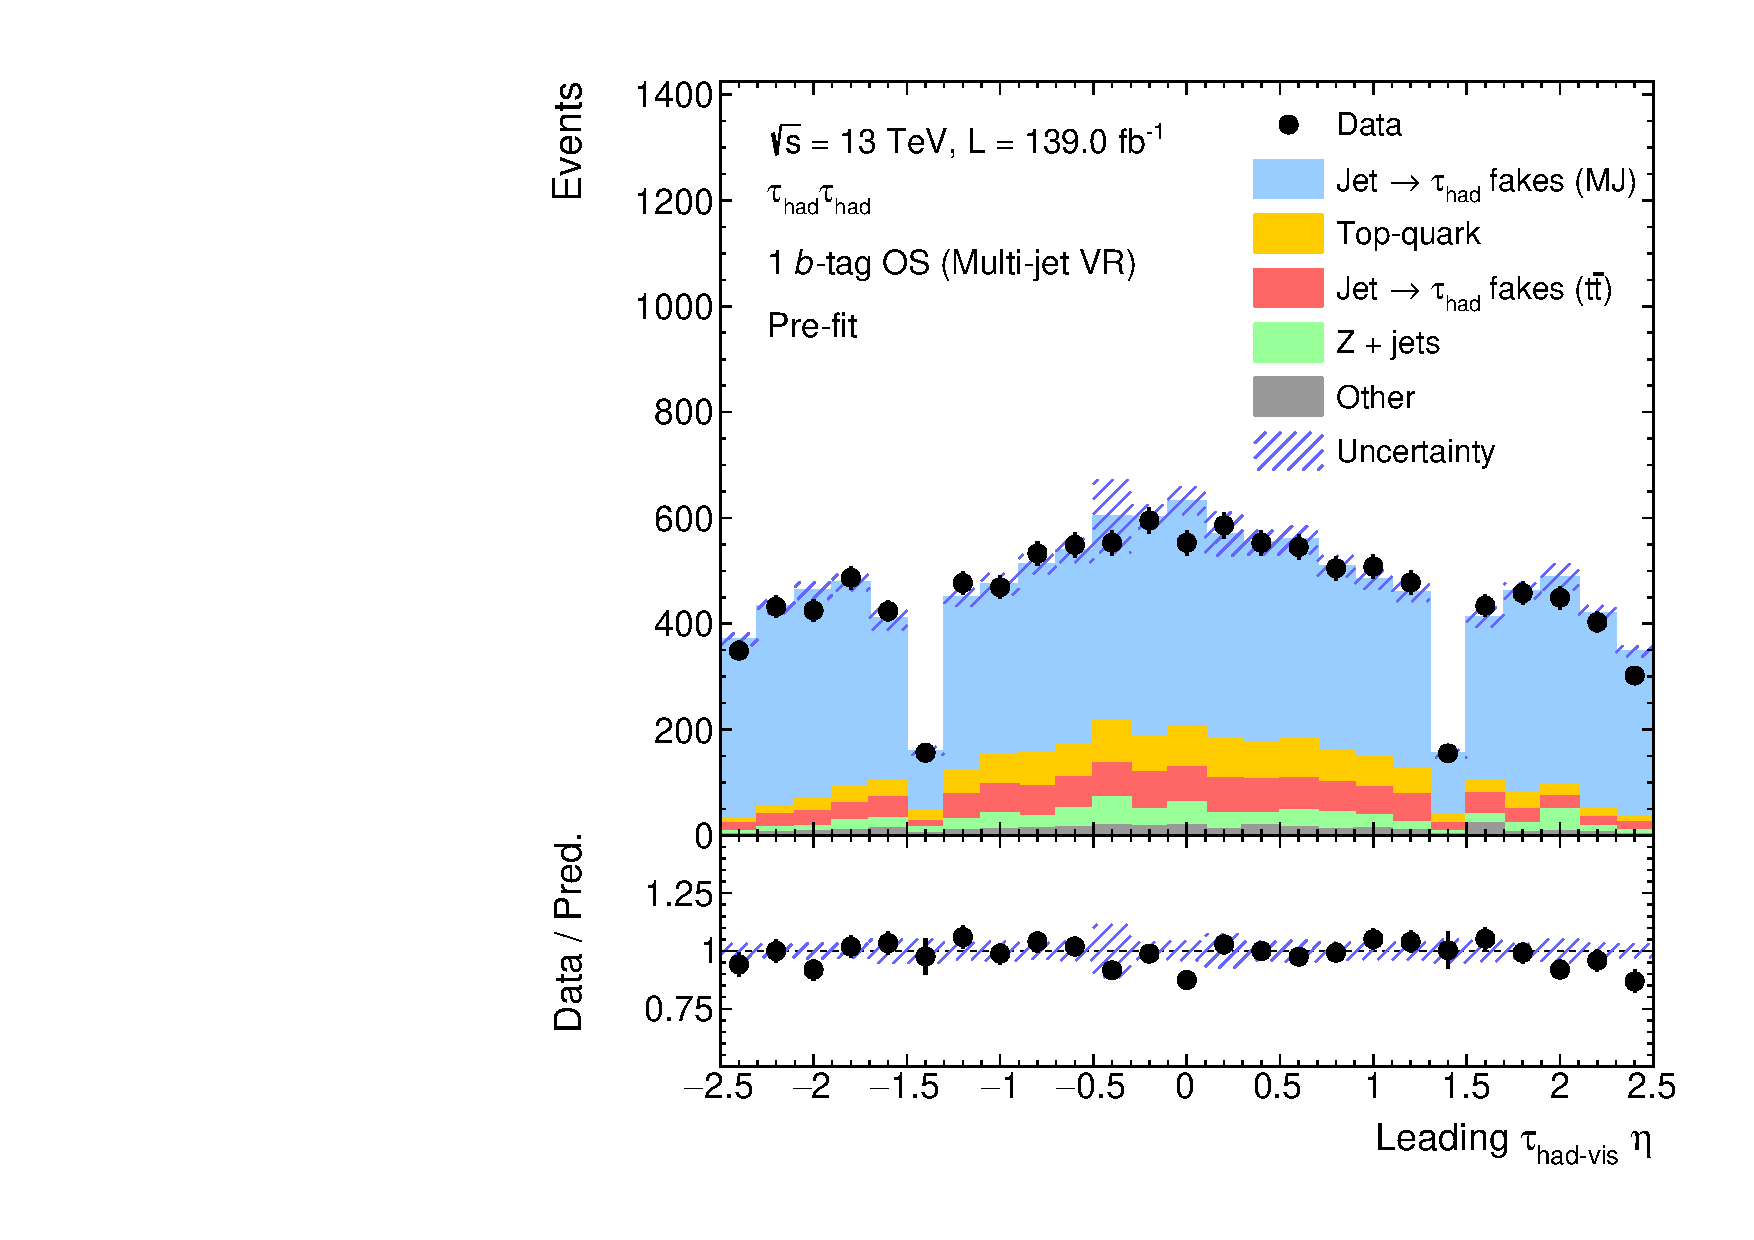
\includegraphics[width=\textwidth]{fakefactors/fake_os_vr/Tau0Eta_fakevr}
  \end{subfigure}\hspace*{0.04\textwidth}%
  \begin{subfigure}{0.45\textwidth}
    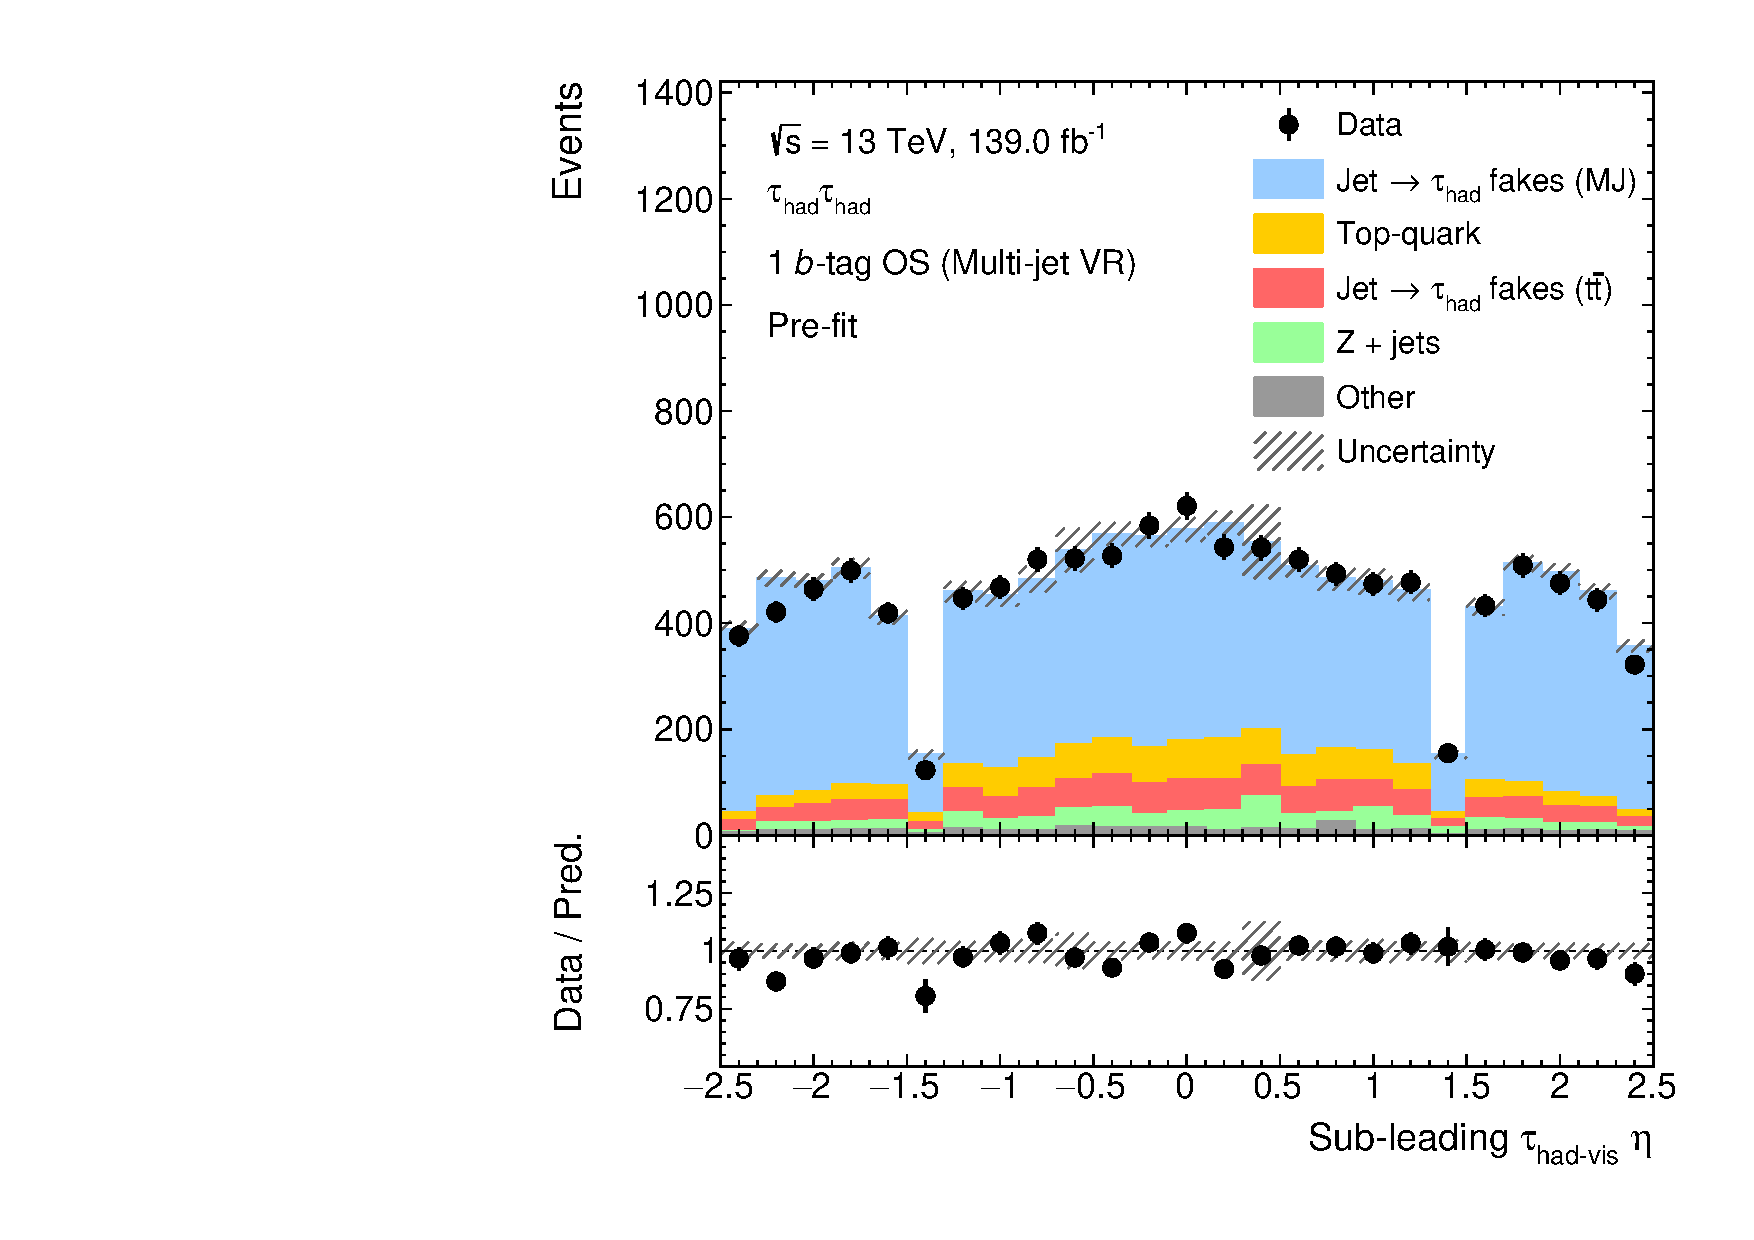
\includegraphics[width=\textwidth]{fakefactors/fake_os_vr/Tau1Eta_fakevr}
  \end{subfigure}

  \begin{subfigure}{0.45\textwidth}
    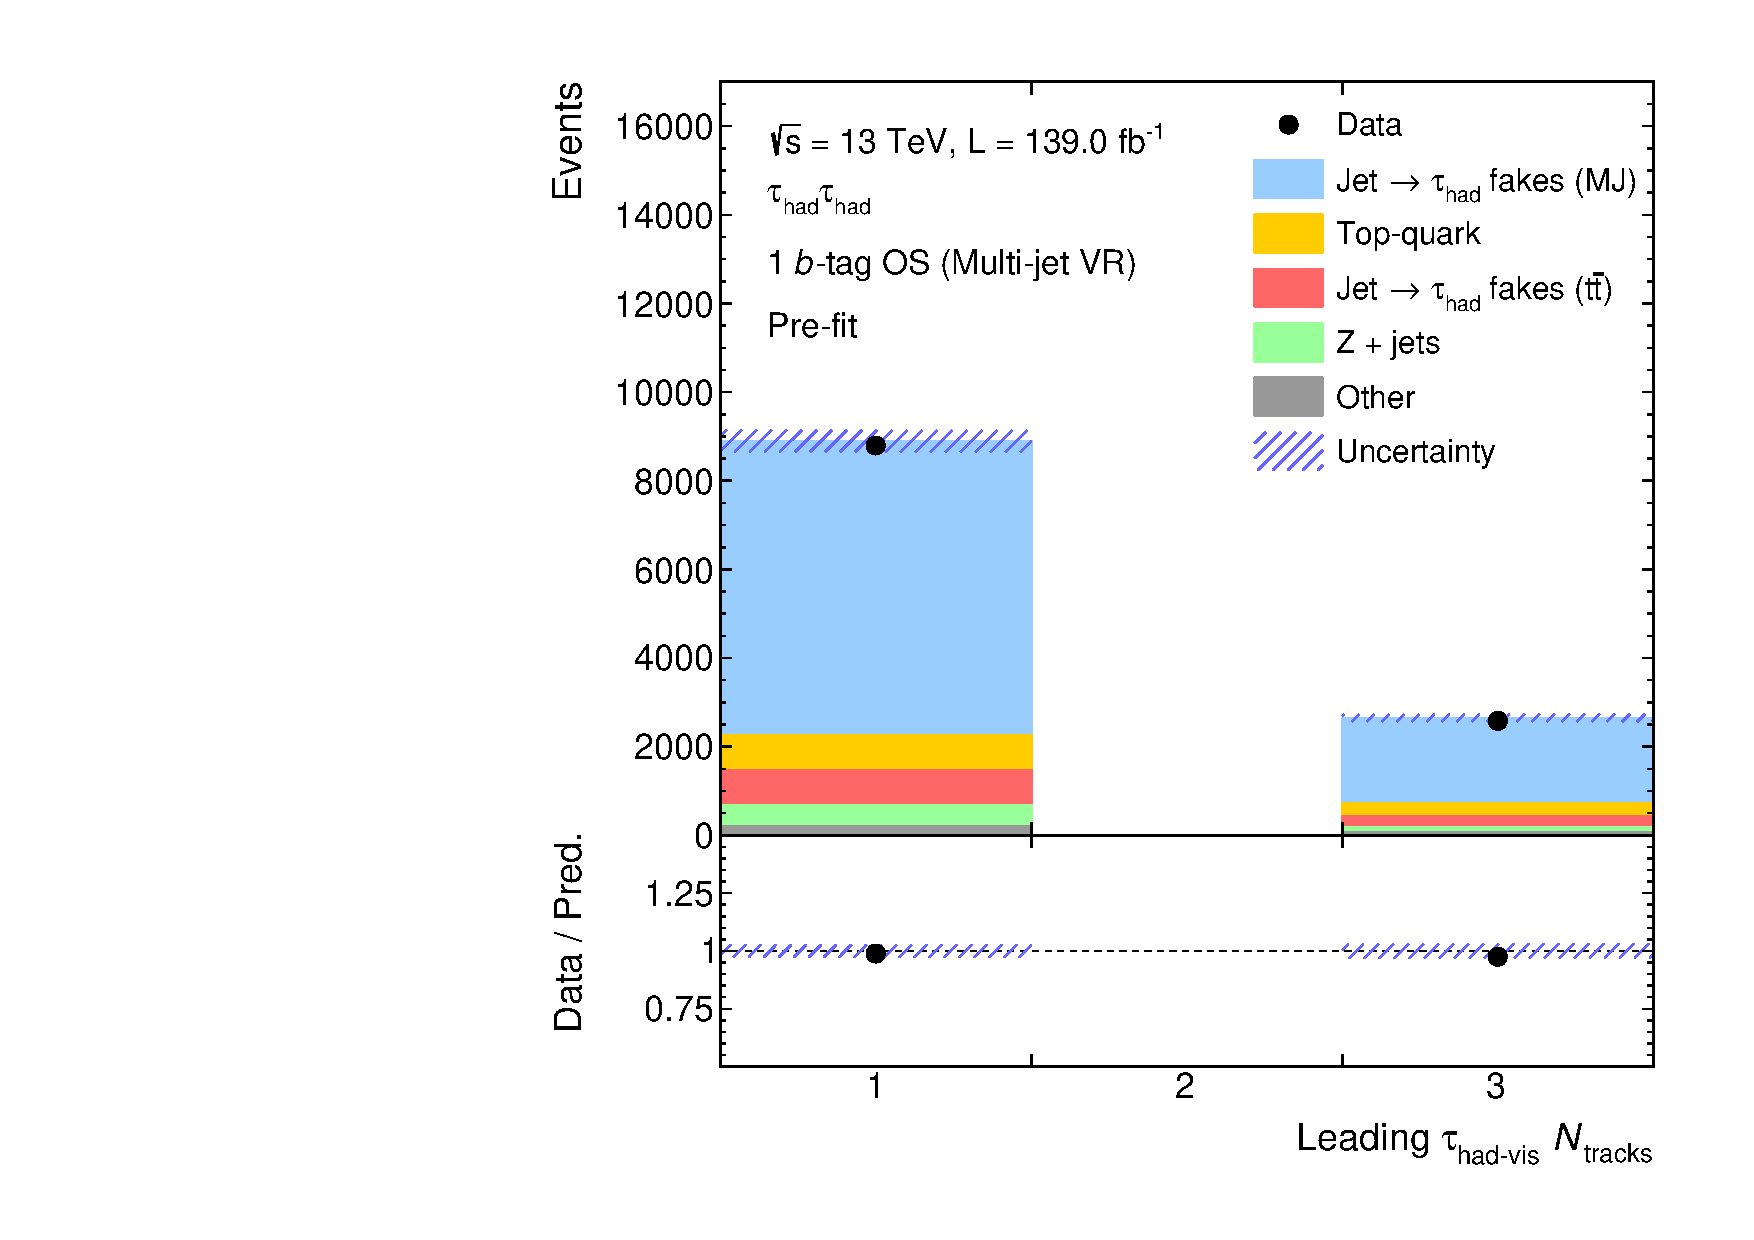
\includegraphics[width=\textwidth]{fakefactors/fake_os_vr/Tau0Ntrk_fakevr}
  \end{subfigure}\hspace*{0.04\textwidth}%
  \begin{subfigure}{0.45\textwidth}
    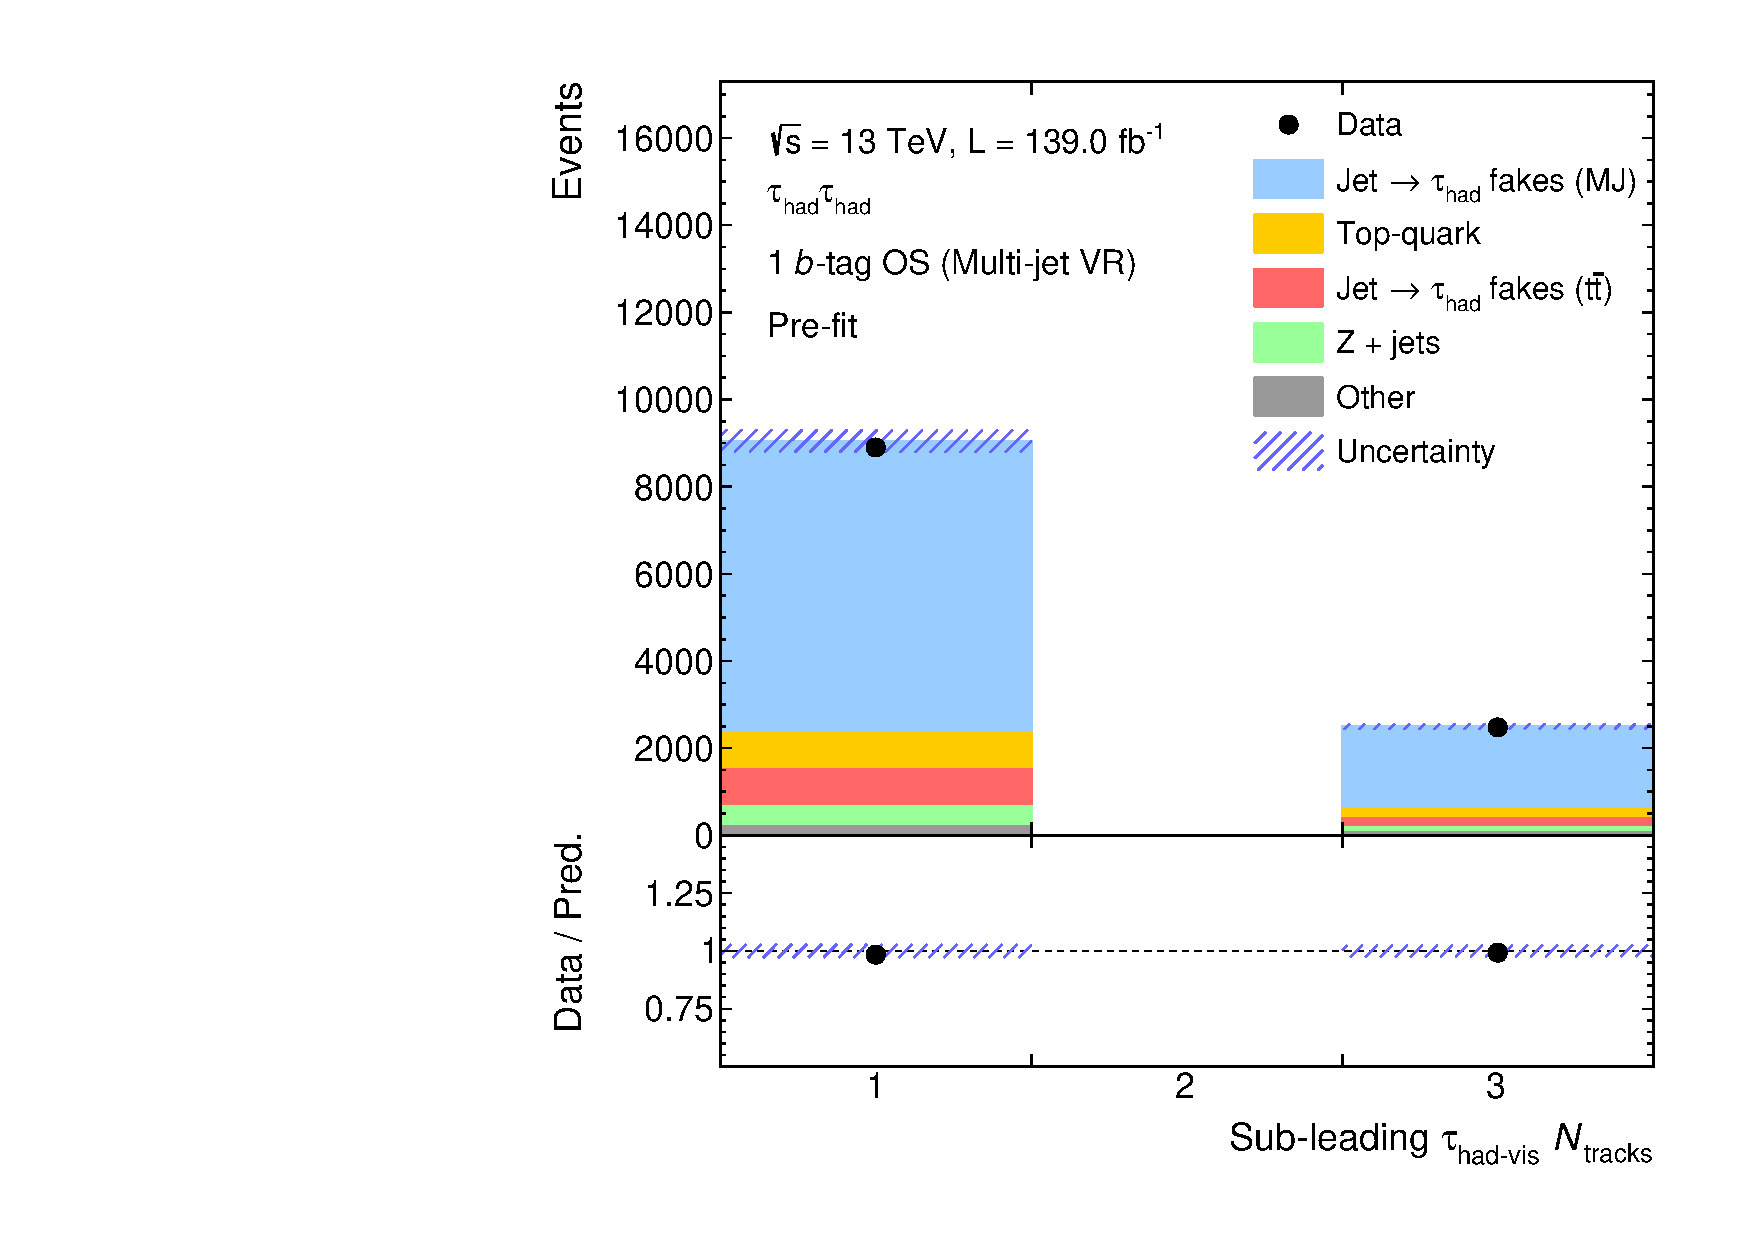
\includegraphics[width=\textwidth]{fakefactors/fake_os_vr/Tau1Ntrk_fakevr}
  \end{subfigure}

  \caption{Validation of \tauhadvis observables in the multi-jet VR (1
    $b$-tag OS, $\mMMC > \SI{110}{\GeV}$, and $\mathcal{S} < 3$). The
    estimate of the multi-jet background (light blue) is obtained
    using the fake factor method (cf.\
    \Cref{fig:fakefactor_regions}). Observables (top: \tauhadvis \pT,
    center: \tauhadvis $\eta$, bottom: \tauhadvis $N_\text{tracks}$)
    of the \tauhadvis candidates leading (left) and sub-leading in \pT
    (right) are shown. The background prediction is shown pre-fit,
    including statistical and detector-related systematic
    uncertainties.}%
  \label{fig:fake_factor_OSVR_kinematics}%
  % Explicitly say that there are no fake uncertainties here yet?
\end{figure}

Further tests of the assumptions can be performed by direct comparison
of fake factors previously measured in the 1 $b$-tag SS region with
the ones that would be obtained from a measurement in the 1 $b$-tag OS
multi-jet VR. Differences between both sets of fake factors can then
be applied as a non-closure uncertainty when applying fake factors
measured in SS regions in OS regions.

In~\Cref{fig:fake_factor_OSSS} a comparison of fake factors measured
in the 1 $b$-tag OS multi-jet VR and the 1 $b$-tag SS region is
shown.

Few events compared to SS and comparatively large subtraction -> large
statistical uncertainties.

The fake factors are compared using $\chi^2$-tests showing good
agreement with one exception. The di-\tauhadvis trigger fake factor
(2015-2016) for 3-prong \tauhadvis with \pT from
\SIrange{50}{65}{\GeV} in the endcaps of the ATLAS detector shows
significant deviations of \SI{50}{\percent} between OS and SS regions.


% Say something regarding the independence?

% Independence -> SS and OS fake factors have to agree
%
% measure OS fake factors in this region and add full difference as an uncertainty.

\begin{figure}[htbp]
  \centering

  \begin{subfigure}[t]{0.48\textwidth}
    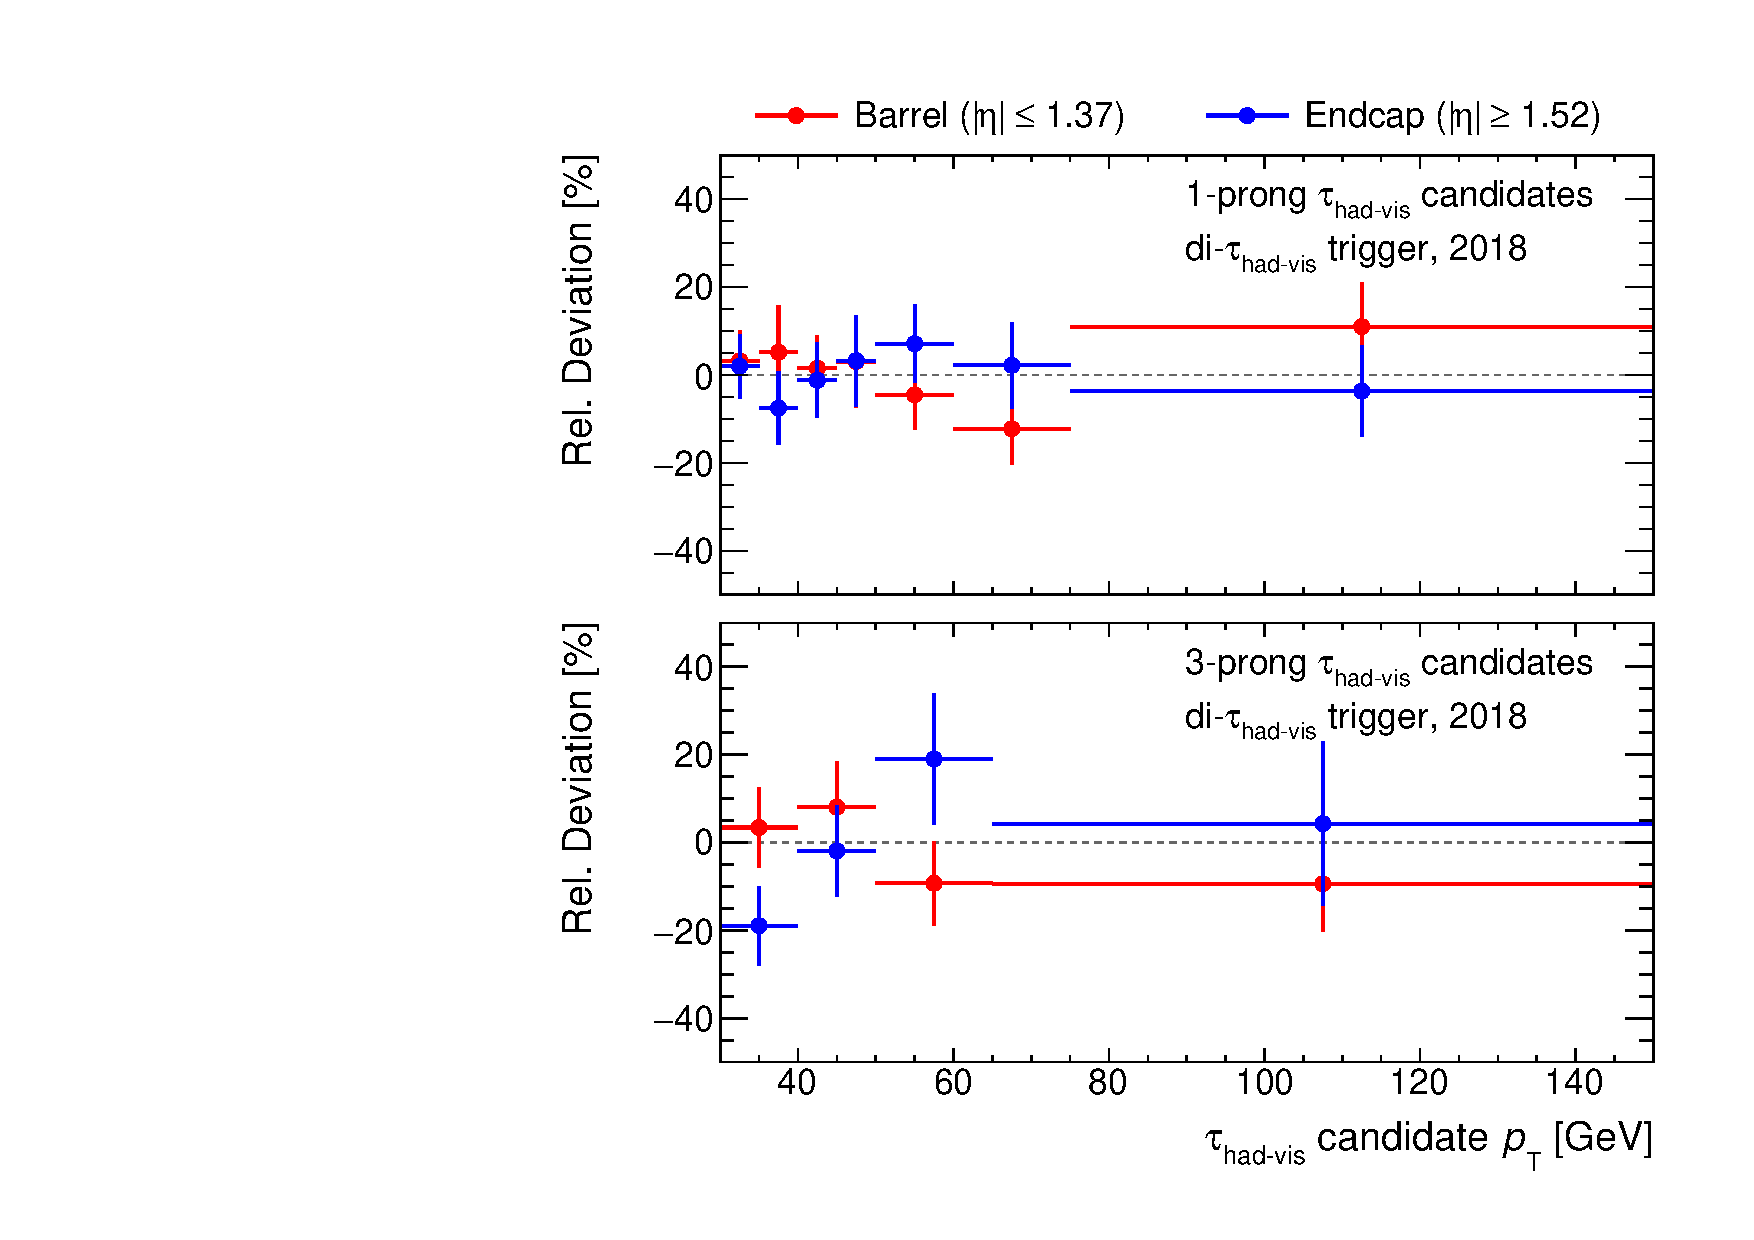
\includegraphics[width=\textwidth]{fakefactors/os_ss/fake_factors_osss_18}
    \subcaption{Comparison of OS and SS fake factors for events
      selected by di-\tauhadvis triggers. Only the 2018 data
      collection period is shown for illustration purposes.}
  \end{subfigure}\hfill%
  \begin{subfigure}[t]{0.48\textwidth}
    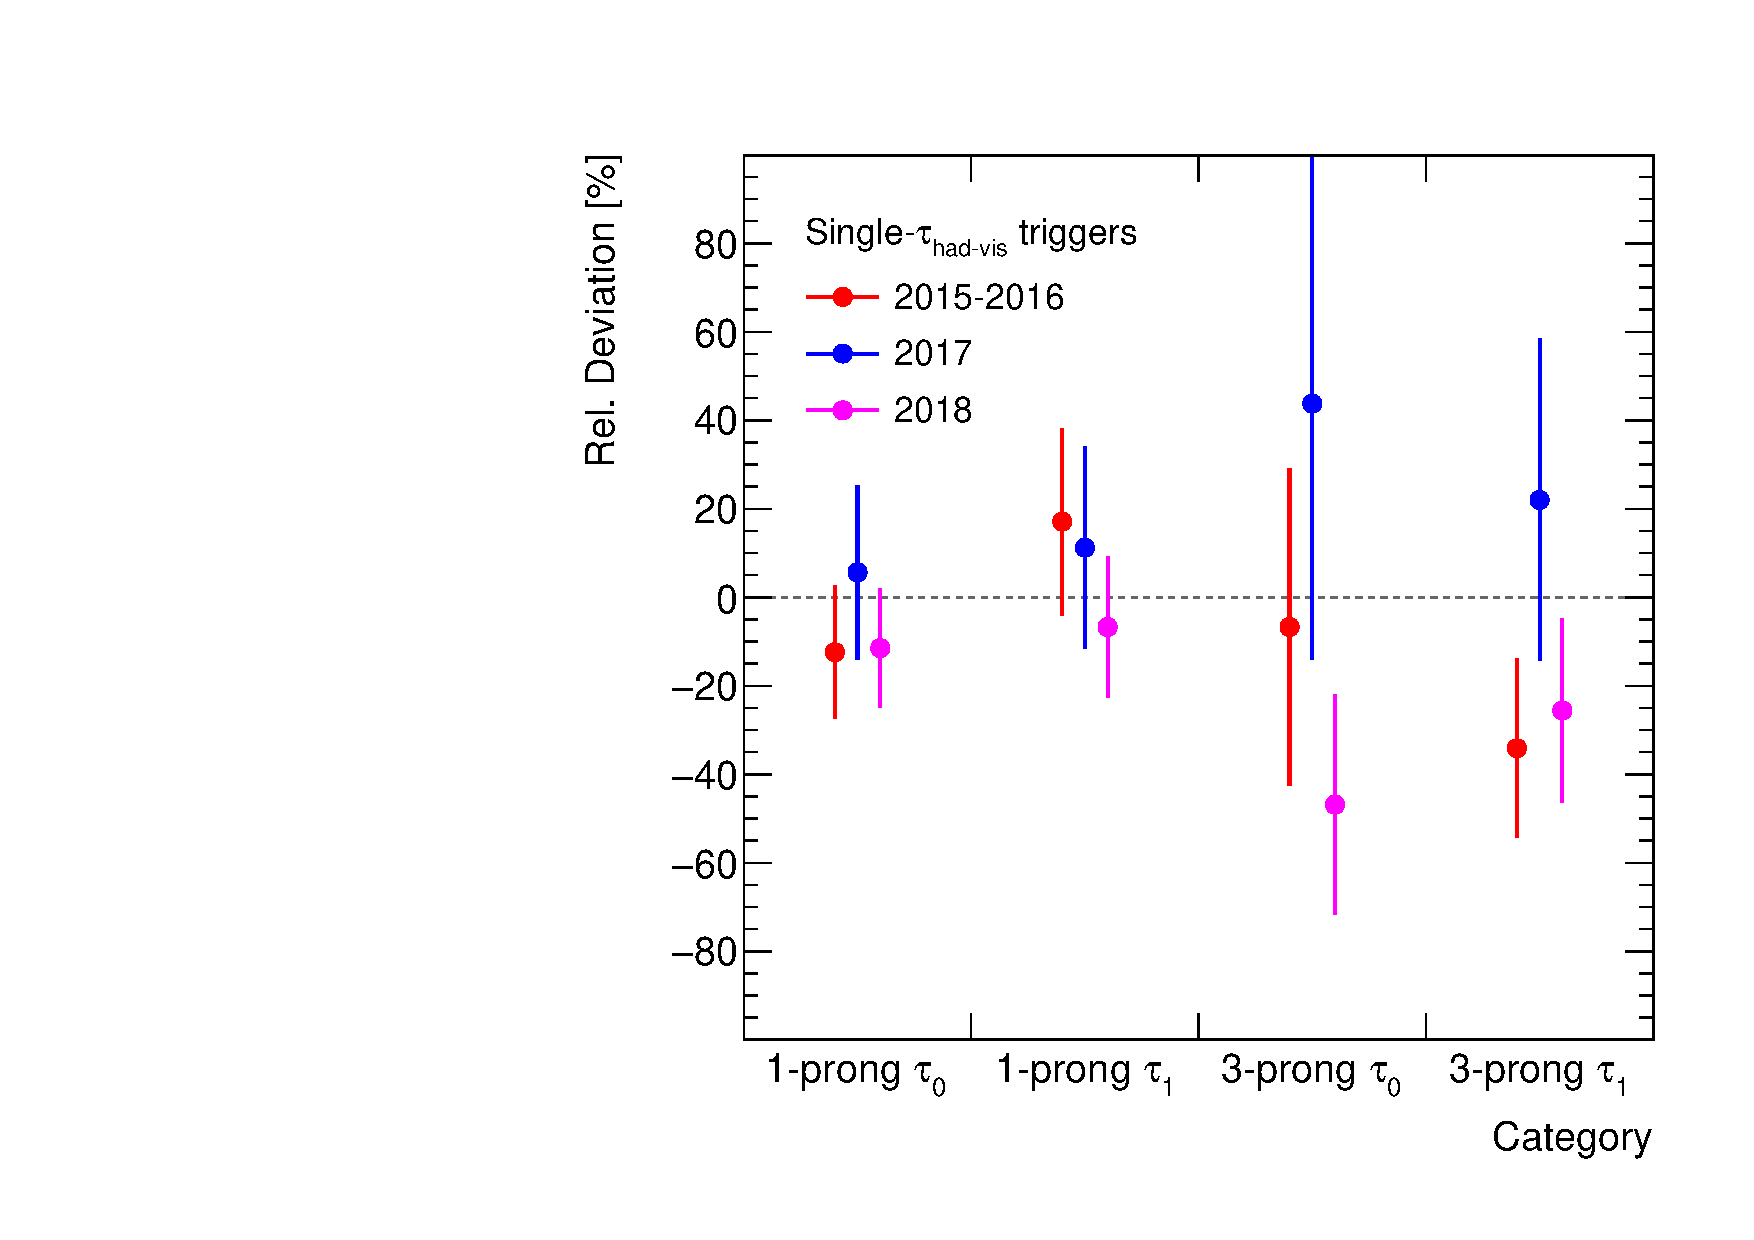
\includegraphics[width=\textwidth]{fakefactors/os_ss/fake_factors_osss_stt}
    \subcaption{Comparison of OS and SS fake factors for events
      selected by single-\tauhadvis triggers for all major data
      collection periods.}
  \end{subfigure}

  \caption{Relative deviation of fake factors measured in the 1
    $b$-tag OS multi-jet VR compared to the nominal set of fake
    factors measured in the 1 $b$-tag SS region (cf.\
    \Cref{fig:mjfakes_fake_factors,fig:mjfakes_stt_ffs}). The relative
    deviation is measured as $\FF_\text{OS} / \FF_\text{SS} - 1$ and
    is used to define a non-closure uncertainty that is propagated to
    the multi-jet background estimate when applying SS fake factors to
    events in OS regions. Statistical uncertainties from the finite
    number of observed data events and the non-multi-jet subtraction
    are shown.}
  \label{fig:fake_factor_OSSS}
\end{figure}



\subsubsection{Estimation of multi-jet backgrounds in the signal region}

% - Transfer factor calculation
% - Subtraction in Anti-ID region

\begin{figure}[htbp]
  \centering

  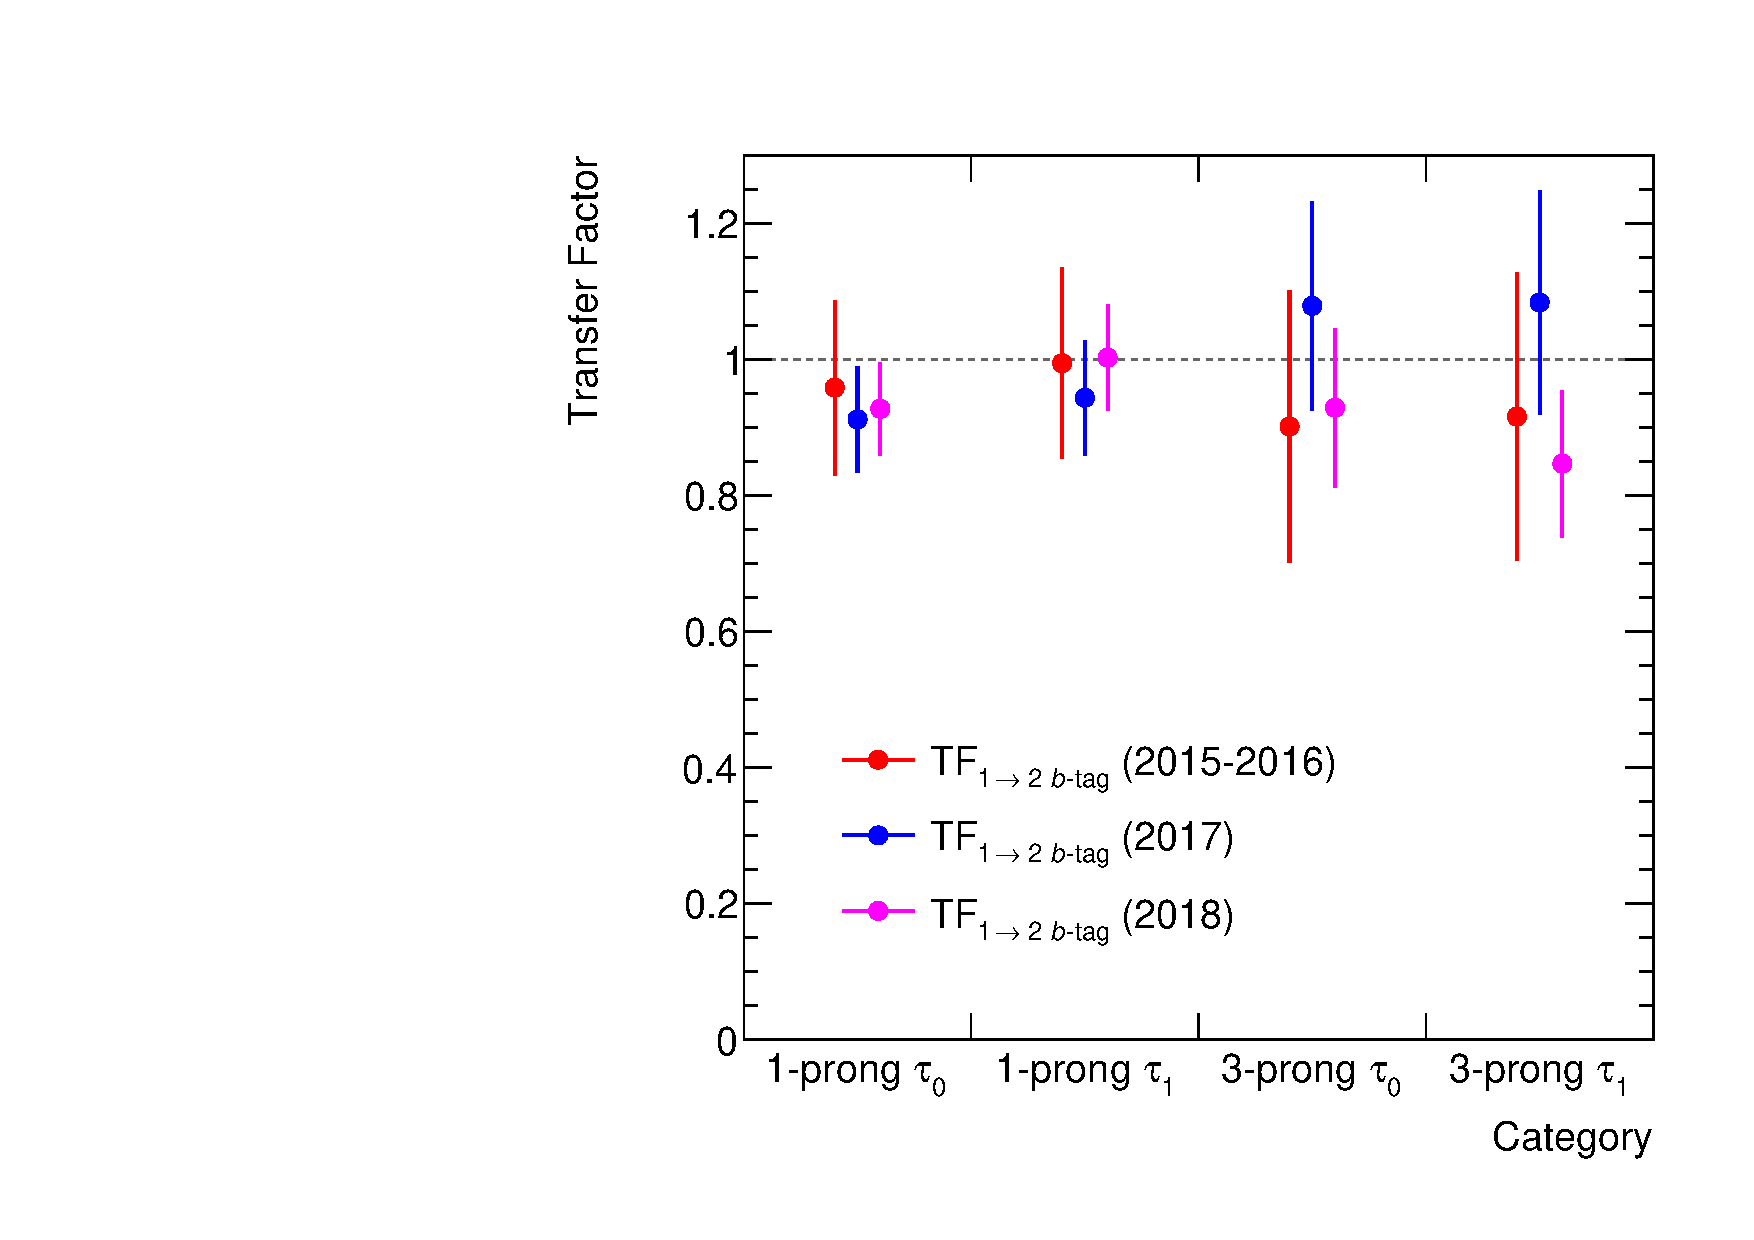
\includegraphics[width=0.495\textwidth]{fakefactors/transfer_factors}

  \caption{Transfer Factors}
  \label{fig:mjfakes_transfer_factor}
\end{figure}


\subsubsection{Transfer factors}

The signal region is in 2 $b$-tag...

% Problems:
%
% - Very few events in SS region and high impurities from ttbar fakes
%   -> Only inclusive fake factors possible
%
%   - Transfer factor is determined by comparing the inclusive fake
%   factor calculated in 1-tag to an inclusive fake factor calculated
%   in 2-tag.
%
%   - Transfer factors show good agremeent between the 1- and 2-tag
%   region with large uncertainties
%
%   - Large uncertainties indicate that we have little sensitivity to
%   the differences between 1- and 2-tag regions.
%
%   - Therefore the 1-tag fake factors are used also in 2-tag region
%   after multiplying them by the transfer factor
%
%   - The primary aim of the transfer factor is to estimate an
%   uncertainty by coherently (conservative approach) varying the
%   transfer factors up and down separate for all four categories.



\subsubsection{Systematic Uncertainties}

% - Uncertainties


% The fake factors are not expected to depend strongly
% on the applied \btag requirement

% Dominant subtraction is ttbar, execpt for 1-tag OS ID where it is
% Ztautau.

% Signal contamination / other background contamination

% Yield table / plots of regions

% Checked in 1-tag OS. Does agreement in 1-tag OS confirm that charge
% and ID are independent? Closure, yes

\todo[inline]{Old stuff below:}

Systematic uncertainties are assigned to cover possible difference
betwen OS and SS fake factors, varying the subtraction in the OS
Anti-ID region. Moreover, the fake factors are independently varied by
their statistical uncertainty.

\todo[inline]{Could we use nOS to enhance statistics? Maybe flip the FF method
  so that we use events in SS ID to build the template instead of OS Anti-ID.}

\todo[inline]{Can we make the STT FF depend on the trigger-match instead of
  the leading / subleading binning?}

%%% Local Variables:
%%% mode: latex
%%% TeX-master: "../../phd_thesis"
%%% End:
